\documentclass[a4paper,11pt]{article}

\usepackage[T1]{fontenc}
\usepackage[utf8]{inputenc}
\usepackage{lmodern}
\usepackage[margin=2.5cm]{geometry}
\usepackage{amsmath,amssymb}
\usepackage{graphicx}
\usepackage{booktabs}
\usepackage{tabularx}
\usepackage{longtable}
\usepackage{array}
\usepackage{xcolor}
\usepackage{listings}
\usepackage{siunitx}
\usepackage{enumitem}
\usepackage{caption}
\PassOptionsToPackage{obeyspaces,spaces,hyphens}{url}
\usepackage[hidelinks]{hyperref}
\urlstyle{tt}
\makeatletter
\g@addto@macro{\UrlBreaks}{\do\_\do\.\do\(\do\)\do\,\do\=\do\/\do\-\do\'}
\makeatother

\sisetup{group-separator={,},group-minimum-digits=4}
\setlist{itemsep=2pt,topsep=4pt}
\captionsetup{font=small,labelfont=bf}
\setlength{\emergencystretch}{2em}

\definecolor{codebg}{RGB}{247,247,245}
\definecolor{codekw}{RGB}{42,120,214}
\definecolor{codecm}{RGB}{110,110,110}
\definecolor{codestr}{RGB}{0,131,0}
\lstdefinestyle{py}{
  language=Python, basicstyle=\ttfamily\footnotesize, backgroundcolor=\color{codebg},
  keywordstyle=\color{codekw}, commentstyle=\color{codecm}\itshape,
  stringstyle=\color{codestr}, showstringspaces=false, breaklines=true,
  frame=single, rulecolor=\color{codebg}, xleftmargin=4pt, xrightmargin=4pt,
  columns=fullflexible, keepspaces=true}
\lstset{style=py}

\newcommand{\code}[1]{\nolinkurl{#1}}
\newcommand{\fn}[1]{\nolinkurl{#1}}
\newcommand{\jdes}{j_\mathrm{des}}
\newcommand{\Vdes}{V_\mathrm{cell,des}}
\newcommand{\Pel}{P_\mathrm{el}}

\title{PhlyGreen Technical Manual: Fuel Cell\\[4pt]
\large Theory, implementation and usage of the PEM fuel-cell system model}
\author{PhlyGreen development team, Sapienza University of Rome}
\date{Code state: November 2026, branch \texttt{main}}

\begin{document}
\maketitle

\begin{abstract}
This manual documents the proton-exchange-membrane (PEM) fuel-cell system model of PhlyGreen.
We derive every equation the code solves, from the analytical polarization curve to the heat
rejected to the coolant. We then describe how the stack is sized, how its operating point is
found at every instant of the mission, and how the fuel cell is closed self-consistently with
the take-off weight. Two further chapters cover the fuel-cell side of the fuel-cell + battery
hybrid and the state-of-health (degradation) model. The last chapters give runnable usage
examples and list the tests that pin each behaviour. Every number in the text comes either
from the code and its parameter database or from running the code; the configuration used is
stated each time. All figures are produced by \fn{manuals/fuel-cell/scripts/make_figures.py}.
\end{abstract}

\tableofcontents
\clearpage

%% =====================================================================================
\section{Scope and position in PhlyGreen}
\label{sec:scope}

This manual covers the fuel-cell \emph{system}: stack, air supply, fixed auxiliaries, the
electric drive that the stack feeds, and the heat the stack generates. Two sibling manuals
cover the neighbouring subsystems. The battery model, including its own state of health, is
documented in \emph{PhlyGreen Technical Manual: Battery}. The rejection of the fuel-cell heat
(Class-I and Class-II thermal-management systems, heat exchangers, ram-air drag) is documented
in \emph{PhlyGreen Technical Manual: Thermal Management}. Here we treat heat
\emph{generation} only and refer to the TMS manual for heat rejection.

\subsection{Configurations that use the fuel cell}

Two values of the \code{Configuration} flag activate the fuel cell.
\begin{itemize}
  \item \code{'Hydrogen'}: a fuel-cell electric aircraft. Hydrogen feeds the stack, the stack
  feeds an electric motor through a power-management and distribution unit (PMAD), and the
  motor drives the propeller through a gearbox. There is no battery and no gas turbine.
  \item \code{'FuelCellBattery'}: the same chain with a battery on the electrical bus. The
  propulsive power is split by the supplied-power ratio $\varphi$ of the mission profile:
  the battery supplies $\varphi$ of it and the fuel cell the remaining $1-\varphi$.
\end{itemize}
A \code{'FuelCellBattery'} design with $\varphi=0$ everywhere is bit-identical to a
\code{'Hydrogen'} design, because both use the same mission integrator form and the same
sizing loop (Section~\ref{sec:closure}).

\subsection{Mediator wiring}

PhlyGreen is organised as a hub-and-spoke object graph. The \code{Aircraft} object
(\fn{trunk/PhlyGreen/Aircraft.py}) holds a reference to every subsystem and every subsystem
holds a reference back to the aircraft. The fuel cell is an optional subsystem: the
constructor \fn{Aircraft.__init__} takes \code{fuelcell=None}, \code{tank=None} and
\code{tms=None}. The factory \fn{trunk/PhlyGreen/factory.py:build_aircraft} always builds a
\code{FuelCell(None)} and a \code{ThermalManagementSystem(None)} and wires them in both
directions, so the attribute \code{aircraft.fuelcell} exists for every configuration. The
fuel cell reads its inputs from \code{aircraft.EnergyInput}, uses \code{aircraft.powertrain}
for the motor and PMAD specific powers, and writes its masses into \code{aircraft.weight}.

Table~\ref{tab:code-map} lists where each part of the model lives.

\begin{table}[ht]
\centering\small
\caption{Code map of the fuel-cell model. Paths are relative to \fn{trunk/PhlyGreen/}.}
\label{tab:code-map}
\begin{tabularx}{\textwidth}{@{}lX@{}}
\toprule
Code & Role \\
\midrule
\fn{Systems/FuelCell/FC_Models.py:FC_Database} & parameter database of three PEM models \\
\fn{Systems/FuelCell/FuelCell.py:FuelCell.PolarizationCurve} & cell voltage, Section~\ref{sec:polcurve} \\
\fn{FuelCell._compute_air_system_power} & compressor and expander, Section~\ref{sec:air} \\
\fn{FuelCell.product_water_vapour_fraction}, \fn{vapour_fraction_at} & phase of the product water, Section~\ref{sec:heat} \\
\fn{FuelCell.cathode_inlet_rh}, \fn{cathode_exhaust} & inlet humidity and exhaust, Sections~\ref{sec:air}, \ref{sec:humidity} \\
\fn{FuelCell._get_env} & ambient state (ISA + DISA) \\
\fn{FuelCell._size_stack} & stack, BoP and drive sizing kernel, Section~\ref{sec:design} \\
\fn{FuelCell.ComputePRatio} & operating point at one flight condition, Section~\ref{sec:operating} \\
\fn{FuelCell.drive_efficiencies} & motor and propeller efficiencies of the drive, Section~\ref{sec:operating} \\
\fn{FuelCell.report_sizing} & power-adequacy report, Section~\ref{sec:adequacy} \\
\fn{FuelCell.set_state_of_health} & degradation state, Section~\ref{sec:degradation} \\
\fn{Mission/Mission.py:Mission.HydrogenConfiguration} & mission integration, pure fuel cell \\
\fn{Mission.FuelCellBatteryConfiguration} & mission integration, FC + Class-I battery \\
\fn{Mission.FuelCellBatteryConfigurationClassII} & mission integration, FC + Class-II battery \\
\fn{Mission._ground_segments} & taxi-out, take-off run and taxi-in \\
\fn{Mission._fuel_cell_chemical_power} & hydrogen power from the stack flow \\
\fn{Mission._takeoff_fc_heat}, \fn{_track_fc_heat_on_solution} & heat points for the TMS \\
\fn{Mission._fc_battery_terminal_power} & battery terminal power (FC + battery) \\
\fn{Weight/Weight.py:Weight.Hydrogen}, \fn{Weight.FuelCellBattery} & take-off-weight closure \\
\fn{Weight._fuel_cell_and_tms_closure} & self-consistent fuel-cell sizing loop \\
\fn{Weight._hydrogen_tank_mass} & tank mass (gravimetric index or LH2 tank) \\
\fn{config/sections.py:EnergyConfig}, \fn{TankConfig}, \fn{MissionConfig} & typed inputs \\
\bottomrule
\end{tabularx}
\end{table}

%% =====================================================================================
\section{Theory}
\label{sec:theory}

This section derives the equations of the fuel-cell system model. We follow the order in
which the code evaluates them at one operating point: cell voltage, air system, net power,
hydrogen flow and heat.

\subsection{Cell voltage: the analytical polarization curve}
\label{sec:polcurve}

The cell voltage is computed by \fn{FuelCell.PolarizationCurve(i_dens, P_internal_Pa, T_amb=None, bol=False)}.
The model is the analytical PEM polarization curve of Kulikovsky~\cite{kulikovsky}, with the
parameter sets of Massaro et al.~\cite{massaro} and an added empirical concentration term.
The database header (\fn{FC_Models.py}) states this origin. The cell voltage at current
density $j$ [\si{A/cm^2}] is
\begin{equation}
  V_\mathrm{cell}(j) = \max\!\Big(10^{-3},\;
  V_\mathrm{oc} - R_\Omega\, j - \eta_0(j) - V_\mathrm{conc}(j) - \Delta V\Big),
  \label{eq:vcell}
\end{equation}
where $V_\mathrm{oc}$ is the open-circuit voltage, $R_\Omega$ the area-specific ohmic
resistance, $\eta_0$ the cathode catalyst-layer (CCL) overpotential, $V_\mathrm{conc}$ an
empirical concentration loss and $\Delta V$ a uniform degradation loss
(Section~\ref{sec:degradation}; zero at beginning of life). The code evaluates the curve at
$j_0=\max(10^{-5}, j)$ to avoid the singularity at zero current. The voltage is floored at
\SI{1}{mV}.

\paragraph{Characteristic scales.} The CCL overpotential is written in dimensionless form.
With the Tafel slope $b$ [V], the CCL proton conductivity $\sigma_t$ [S/cm], the CCL
thickness $l_t$ [cm], the volumetric exchange current density $i_*$ [\si{A/cm^3}], the
Faraday constant $F=\SI{96485.33}{C/mol}$ and the reference oxygen concentration
$c_\mathrm{ref}$ [\si{mol/cm^3}], the code defines
\begin{equation}
  j_* = \frac{\sigma_t b}{l_t}, \qquad
  D_* = \frac{\sigma_t b}{4 F c_\mathrm{ref}}, \qquad
  \varepsilon = \sqrt{\frac{\sigma_t b}{2 i_* l_t^2}} ,
\end{equation}
and the dimensionless variables
\begin{equation}
  \tilde j = \frac{j_0}{j_*}, \qquad
  \tilde c_h = \frac{c_h}{c_\mathrm{ref}}, \qquad
  \tilde D = \frac{D_\mathrm{CCL}}{D_*}, \qquad
  c_h = c_{h,\mathrm{ref}}\,\frac{p}{\SI{1}{bar}} ,
\end{equation}
where $D_\mathrm{CCL}$ [\si{cm^2/s}] is the CCL oxygen diffusivity and $c_h$ the oxygen
concentration in the channel, proportional to the cathode pressure $p$ (the code passes
\code{Target_Press}). The gas-diffusion layer (GDL) has a limiting current density
\begin{equation}
  j_\mathrm{lim}^{*} = \frac{4 F D_b c_h}{l_b}, \qquad
  r = \min\!\Big(\frac{j_0}{j^*_\mathrm{lim}},\, 0.999\Big),
\end{equation}
with $D_b$ [\si{cm^2/s}] the GDL diffusivity and $l_b$ [cm] its thickness. The cap at 0.999
keeps the logarithms finite.

\paragraph{CCL overpotential.} With the auxiliary function
\begin{equation}
  \beta_\mathrm{K}(\tilde j) = \frac{\sqrt{2\tilde j}}{1+\sqrt{1.12\,\tilde j}\;\exp\!\big(\sqrt{2\tilde j}\big)}
  + \frac{\pi \tilde j}{2+\tilde j},
\end{equation}
the overpotential is $\eta_0 = b\,\tilde\eta_0$ with
\begin{equation}
  \tilde\eta_0 =
  \underbrace{\operatorname{arcsinh}\!\left(\frac{\varepsilon^2\tilde j^2}
      {2\tilde c_h\,\big(1-e^{-\tilde j/2}\big)}\right)}_{\text{(I) kinetics}}
  + \underbrace{\frac{1}{\tilde c_h \tilde D}\,
      \frac{\tilde j - \ln\!\big(1+\tilde j^2/\beta_\mathrm{K}^2\big)}{1-r}}_{\text{(II) CCL O$_2$ transport}}
  \underbrace{-\,\ln(1-r)}_{\text{(III) GDL transport}} .
  \label{eq:eta0}
\end{equation}
Term (I) is the activation overpotential of the oxygen-reduction reaction in a catalyst layer
of finite proton conductivity. Term (II) is the loss due to oxygen diffusion through the CCL,
amplified as the GDL approaches its limiting current. Term (III) is the GDL transport loss.
This attribution follows the structure of the formula and the user guide
(\fn{docs/user-guide/hydrogen.md}, ``activation + O$_2$ transport''); the code itself does not
label the terms.

\paragraph{Empirical concentration loss.} The database adds a concentration term that is not
part of the analytical model. The database comments state that it was tuned to reproduce a
measured flooding knee at high current (\fn{FC_Models.py}, ``Correzioni empiriche'').
\begin{equation}
  V_\mathrm{conc}(j) = \begin{cases}
  -B\,\ln\!\big(1 - j_0/j_\mathrm{lim}\big), & j_0 < j_\mathrm{lim},\\
  \SI{2.5}{V}, & j_0 \ge j_\mathrm{lim},
  \end{cases}
\end{equation}
with $B$ [V] the concentration coefficient (\code{B_conc}) and $j_\mathrm{lim}$
[\si{A/cm^2}] an empirical limiting current density (\code{j_lim}). The constant
\SI{2.5}{V} is a penalty that drives the cell voltage to the \SI{1}{mV} floor beyond
$j_\mathrm{lim}$. Note that $j_\mathrm{lim}$ is distinct from the GDL limiting current
$j^*_\mathrm{lim}$; in the database models $j_\mathrm{lim} < j^*_\mathrm{lim}$, so the
empirical term sets the end of the curve.

\paragraph{What the curve does not depend on.} The argument \code{T_amb} is accepted but
unused. The operating temperature \code{T_op} of the database does not enter
Eq.~\eqref{eq:vcell}: it is used only by the expander (Section~\ref{sec:air}) and by the
product-water phase model (Section~\ref{sec:heat}). Humidity and membrane water content do
not enter either. These are model assumptions.

\paragraph{Database.} Table~\ref{tab:db} lists the three models of \fn{FC_Database} with
their units, and the derived scales computed from them at the database cathode pressure of
\SI{1.5}{bar}. A database model holds only electrochemical and operating parameters. The
design choices of a stack (design cell voltage, stack specific power, BoP mass ratio) are
design inputs of \code{EnergyConfig} (Section~\ref{sec:inputs}).

\begin{table}[ht]
\centering\small
\caption{Parameters of \fn{FC_Database} (\fn{Systems/FuelCell/FC_Models.py}) and derived
quantities computed by \fn{make_figures.py} (group \code{cell}) at $p=\SI{1.5}{bar}$. The
comments in the database cite Massaro et al.\ Table~7 (GoodPerformance) and Table~10
(HighPerformance).}
\label{tab:db}
\begin{tabular}{@{}llrrr@{}}
\toprule
Symbol (key) & Unit & GoodPerformance & HighPerformance & Generic \\
\midrule
$V_\mathrm{oc}$ (\code{Voc}) & V & 1.145 & 1.145 & 1.145 \\
$b$ (\code{b_tafel}) & V & 0.030 & 0.030 & 0.04 \\
$R_\Omega$ (\code{R_ohm}) & \si{\ohm.cm^2} & 0.0801 & 0.0978 & 0.15 \\
$i_*$ (\code{i_star}) & \si{A/cm^3} & \num{2.00e-3} & \num{1.75e-2} & \num{5e-3} \\
$j_\mathrm{lim}$ (\code{j_lim}) & \si{A/cm^2} & 1.65 & 3.0 & 2.5 \\
$B$ (\code{B_conc}) & V & 0.075 & 0.05 & 0.1 \\
$c_{h,\mathrm{ref}}$ (\code{c_h_ref}) & \si{mol/cm^3} & \num{7.36e-6} & \num{7.36e-6} & \num{7.36e-6} \\
$c_\mathrm{ref}$ (\code{c_ref}) & \si{mol/cm^3} & \num{8.58e-6} & \num{8.583e-6} & \num{8.58e-6} \\
$\sigma_t$ (\code{sigma_t}) & S/cm & 0.03 & 0.03 & 0.03 \\
$l_t$ (\code{l_t}) & cm & 0.0007 & 0.0007 & 0.0007 \\
$D_b$ (\code{D_b}) & \si{cm^2/s} & 0.0259 & 0.0259 & 0.0259 \\
$l_b$ (\code{l_b}) & cm & 0.0312 & 0.0188 & 0.0312 \\
$D_\mathrm{CCL}$ (\code{D_ccl}) & \si{cm^2/s} & \num{1.00e-4} & \num{1.40e-4} & \num{1.00e-4} \\
$T_\mathrm{op}$ (\code{T_op}) & K & 353.15 & 443.15 & 353.15 \\
$p$ (\code{Target_Press}) & Pa & \num{150000} & \num{150000} & \num{150000} \\
\midrule
$j_*$ & \si{A/cm^2} & 1.286 & 1.286 & 1.714 \\
$\varepsilon$ & -- & 678 & 229 & 495 \\
$\tilde D$ & -- & 0.368 & 0.515 & 0.276 \\
$j^*_\mathrm{lim}$ & \si{A/cm^2} & 3.54 & 5.87 & 3.54 \\
$V_\mathrm{cell}(\SI{e-4}{A/cm^2})$ & V & 1.024 & 1.089 & 1.021 \\
$j$ at \SI{0.7}{V} & \si{A/cm^2} & 0.421 & 0.801 & 0.135 \\
$j$ at \SI{0.5}{V} & \si{A/cm^2} & 1.147 & 1.809 & 0.660 \\
max.\ $jV$ & \si{W/cm^2} & 0.579 & 0.917 & 0.386 \\
$j$, $V$ at max.\ $jV$ & \si{A/cm^2}, V & 1.24, 0.466 & 2.02, 0.455 & 1.05, 0.368 \\
\bottomrule
\end{tabular}
\end{table}

Figure~\ref{fig:polarization} shows the three curves and their power densities.
Figure~\ref{fig:losses} splits the losses of the reference model. The CCL term $\eta_0$
dominates everywhere. At \SI{0.1}{A/cm^2} it is already \SI{0.33}{V}, against
\SI{0.008}{V} of ohmic loss; at the reference design point (\SI{1.147}{A/cm^2},
\SI{0.5}{V}) the three losses are \SI{0.464}{V}, \SI{0.092}{V} and \SI{0.089}{V}. Note that
every database model has its maximum power density below \SI{0.47}{V}.

\begin{figure}[ht]
\centering
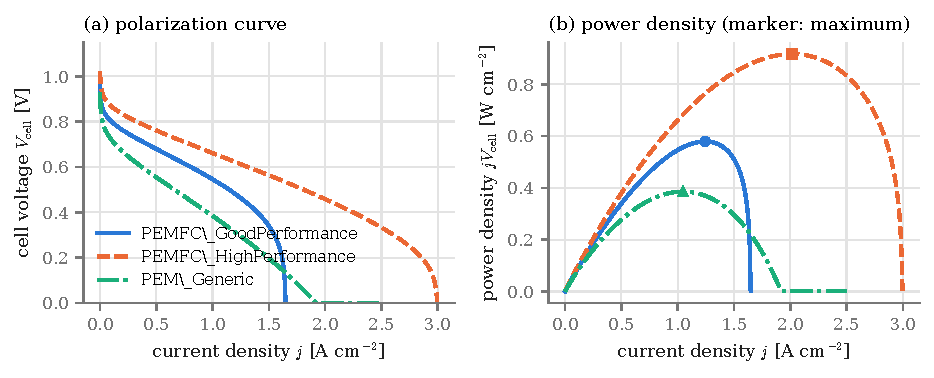
\includegraphics[width=\textwidth]{figures/fig_polarization.pdf}
\caption{Polarization curves (a) and power densities (b) of the three database models at
\SI{1.5}{bar}, beginning of life. Markers in (b) give the maximum power density. Produced by
\fn{make_figures.py:group_cell}.}
\label{fig:polarization}
\end{figure}

\begin{figure}[ht]
\centering
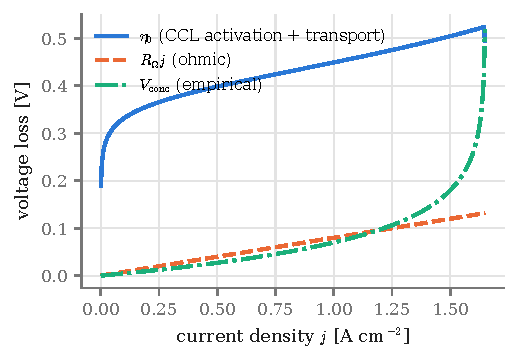
\includegraphics[width=0.55\textwidth]{figures/fig_losses.pdf}
\caption{Voltage losses of \code{PEMFC_GoodPerformance} at \SI{1.5}{bar}: CCL overpotential
$\eta_0$ of Eq.~\eqref{eq:eta0}, ohmic loss and empirical concentration loss. Their sum
plus $V_\mathrm{cell}$ equals $V_\mathrm{oc}=\SI{1.145}{V}$.}
\label{fig:losses}
\end{figure}

\subsection{Air system: compressor and expander}
\label{sec:air}

The cathode is held at the constant pressure $p_c=$ \code{Target_Press} at every altitude.
The ambient air is compressed from $p_a(h)$ to $p_c$, and the cathode exhaust is expanded back
to ambient through a turbine (expander). The model is
\fn{FuelCell._compute_air_system_power(P_amb, T_amb, I_tot)}.

\paragraph{Ambient state.} \fn{FuelCell._get_env(alt)} returns the ambient pressure and
temperature of the package ISA model, $p_a=$ \fn{atmosphere.Pstd}$(h)$ and
$T_a=$ \fn{atmosphere.Tstd}$(h)+\Delta T_\mathrm{ISA}$ (\fn{Utilities/Atmosphere.py}), with
$\Delta T_\mathrm{ISA}$ the mission temperature deviation \code{mission.DISA}, read from the
input \code{MissionConfig.disa} (\code{MissionInput['DISA']}, default 0). A hot day therefore
changes the compressor work. The pressure at a given altitude is the standard one.

\paragraph{Compressor.} The dry-air mass flow is
\begin{equation}
  \dot m_\mathrm{air,dry} = 3.57\times10^{-7}\; N_\mathrm{cells}\, I\, \lambda
  \quad [\si{kg/s}],
  \label{eq:mair}
\end{equation}
where $I=jA_\mathrm{cell}$ is the stack current [A], $N_\mathrm{cells}$ the number of cells
and $\lambda$ the air stoichiometric ratio (\code{stoich}, default 2.0). The coefficient in
kg/(A\,s) is hard-coded; the code comment identifies it as $\dot n_{\mathrm{H_2}}\cdot
0.5\lambda/0.21\cdot M_\mathrm{air}$ per unit $\lambda$, and indeed
$M_\mathrm{air}/(4F\,x_{\mathrm{O_2}}) = 0.02897/(4\cdot96485\cdot0.21) = \SI{3.57e-7}{kg/(A.s)}$.
The compressor takes humid ambient air. With $y_w$ the water mole fraction of the ambient air
(Section~\ref{sec:humidity}),
\begin{gather}
  \dot m_\mathrm{comp} = \dot m_\mathrm{air,dry}\left(1+\frac{y_w}{1-y_w}\,
  \frac{M_{\mathrm{H_2O}}}{M_\mathrm{air}}\right), \\
  P_\mathrm{comp} = \frac{\dot m_\mathrm{comp}\, c_p\, T_a\, \big(\Pi^{0.286}-1\big)}{\eta_\mathrm{comp}},
  \qquad \Pi = \max\!\Big(\frac{p_c}{p_a},1\Big),
\end{gather}
with the dry-air $c_p=\SI{1004}{J/(kg.K)}$ (the water is a small fraction), $M_\mathrm{air}=
\SI{0.02897}{kg/mol}$, $\eta_\mathrm{comp}=0.75$ and the exponent $0.286\approx(\gamma-1)/\gamma$
for $\gamma=1.4$. If $p_c\le p_a$ the air system draws no power. For $p_c=\SI{1.5}{bar}$ the
compressor runs at every altitude, including sea level.

\paragraph{Expander.} The expander takes the cathode exhaust, not the inlet air
(\fn{FuelCell.cathode_exhaust}). Per mole of hydrogen reacted, the exhaust holds
\begin{equation}
  n_{\mathrm{N_2}} = 0.5\lambda\,\frac{0.79}{0.21}, \qquad
  n_{\mathrm{O_2}} = 0.5(\lambda-1), \qquad
  n_{\mathrm{H_2O}} = n_{w,\mathrm{in}} + x_v ,
  \label{eq:exhaust}
\end{equation}
where $n_{w,\mathrm{in}}$ is the water brought by the inlet air at the cathode inlet humidity
and $x_v$ the product water that leaves as vapour (Section~\ref{sec:heat}); the liquid product
water is assumed separated before the expander. With the molar heat capacities
$c_{p,k}$ = 29.12 (N$_2$), 29.38 (O$_2$) and 33.58 (H$_2$O) \si{J/(mol.K)}, the molar masses
$M_k$ = 28.013, 31.999 and \SI{18.015e-3}{kg/mol} (\code{CP_MOLAR}, \code{MOLAR_MASS}) and
$R=\SI{8.3145}{J/(mol.K)}$ (\code{R_GAS}), the mixture properties are
\begin{equation}
  n = \sum_k n_k,\qquad
  \bar c_p = \frac{1}{n}\sum_k n_k c_{p,k},\qquad
  \bar M = \frac{1}{n}\sum_k n_k M_k,\qquad
  \dot m_\mathrm{exh} = \dot n_{\mathrm{H_2}}\, n\, \bar M ,
\end{equation}
with $\dot n_{\mathrm{H_2}} = N_\mathrm{cells}I/2F$. The expander power is
\begin{equation}
  P_\mathrm{turb} = \dot m_\mathrm{exh}\,\frac{\bar c_p}{\bar M}\, T_\mathrm{op}
  \left(1-\Big(\frac{p_a}{0.95\,p_c}\Big)^{R/\bar c_p}\right)\eta_\mathrm{turb}
  \quad \text{if } 0.95\,p_c > p_a ,
\end{equation}
with $\eta_\mathrm{turb}=0.70$. The expander inlet is at the stack temperature and at
\SI{95}{\percent} of the cathode pressure. The net air-system power is
\begin{equation}
  P_\mathrm{comp,net} = \max\big(P_\mathrm{comp}-P_\mathrm{turb},\,0\big).
\end{equation}
The constants $c_{p,k}$ are model constants (``ideal-gas molar heat capacities near the stack
temperature'', code comment). The compressor is supplied directly by the stack: there is no
motor or inverter efficiency in the air-system chain. The efficiencies are constant: there are
no compressor or turbine maps.


\subsection{Net power, hydrogen flow and system efficiency}
\label{sec:netpower}

\paragraph{Electrical power.}
The gross electrical power generated by the stack is reduced by the
net compressor power and the fixed auxiliary loads:
\begin{equation}
  P_\mathrm{gross} = N_\mathrm{cells} V_\mathrm{cell} I, \qquad
  P_\mathrm{fix} = 0.015\,P_\mathrm{fc,rated}, \qquad
  P_\mathrm{net} = P_\mathrm{gross} - P_\mathrm{comp,net} - P_\mathrm{fix}.
  \label{eq:pnet}
\end{equation}
The fixed auxiliary load (\code{Fixed_Aux_Load} = 0.015) is a constant
fraction of the rated power $P_\mathrm{fc,rated}$ (Section~\ref{sec:design}).
Since it does not vary with load, its relative contribution increases
at part-load operation.

\paragraph{Hydrogen consumption.}
The hydrogen mass flow is determined directly from Faraday's law.
Since the oxidation of one hydrogen molecule releases two electrons,
the hydrogen consumed by the stack is
\begin{equation}
  \dot m_{\mathrm{H_2}} =
  \frac{N_\mathrm{cells} I}{2F}\,M_{\mathrm{H_2}},
  \qquad
  M_{\mathrm{H_2}} = \SI{2.016e-3}{kg/mol}.
  \label{eq:mh2}
\end{equation}
This expression assumes unit Faradaic efficiency and neglects additional
hydrogen losses, such as purging and crossover. The electrochemical
hydrogen consumption depends on the stack current, irrespective of
whether the product water leaves the cell in liquid or vapour form.

\paragraph{Chemical power and electrical efficiency.}
The chemical power associated with the consumed hydrogen is evaluated
using its higher heating value (HHV):
\begin{equation}
  P_\mathrm{chem} = \dot m_{\mathrm{H_2}}\,\mathrm{HHV},
  \qquad
  \mathrm{HHV} = \frac{\Delta H_\mathrm{HHV}}{M_{\mathrm{H_2}}}
  = \frac{\SI{286000}{J/mol}}{\SI{2.016e-3}{kg/mol}}
  = \SI{141.87}{MJ/kg}.
\end{equation}
The HHV corresponds to the standard reaction enthalpy of hydrogen
oxidation with liquid product water at the reference conditions.
Its use here defines a fixed reference for the chemical energy input;
it does not imply that all the water actually leaves the operating
stack in the liquid state.

The net fuel-cell-system electrical efficiency is defined as
\begin{equation}
  \eta_\mathrm{FCS} = \frac{P_\mathrm{net}}{P_\mathrm{chem}}.
  \label{eq:etafcs}
\end{equation}
Combining this definition with Faraday's law gives, for
$P_\mathrm{net}>0$,
\begin{equation}
  \dot m_{\mathrm{H_2}}
  = \frac{P_\mathrm{net}}{\eta_\mathrm{FCS}\,\mathrm{HHV}}
  = \frac{N_\mathrm{cells} I}{2F}\,M_{\mathrm{H_2}}.
\end{equation}
Thus, hydrogen consumption calculated from net electrical power and
efficiency is identical to that obtained directly from the current,
provided that the same heating-value reference is used consistently.
In the present model, efficiency is calculated from the hydrogen
consumption rather than prescribed independently.

An LHV-based efficiency could equally be defined, but it would have
a different numerical value. The corresponding product of efficiency
and heating value would remain unchanged:
\begin{equation}
  \eta_\mathrm{FCS,HHV}\,\mathrm{HHV}
  = \eta_\mathrm{FCS,LHV}\,\mathrm{LHV}
  = \frac{P_\mathrm{net}}{\dot m_{\mathrm{H_2}}}.
\end{equation}
Consequently, the choice of heating-value reference does not affect
the hydrogen consumption when applied consistently.

\paragraph{Consistency with the water-phase model.}
At the operating temperature of a PEM fuel cell, the product water
may leave partly or entirely as vapour, depending on the cathode
air flow, pressure and humidity. Evaporation carries part of the
reaction energy into the exhaust stream, reducing the heat that must
be removed by the coolant.

This effect is accounted for separately in Section~\ref{sec:heat}
through the product-water vapour fraction $x_v$. The electrical
efficiency retains the fixed HHV reference, whereas the thermal
balance accounts for the actual water phase. At fixed stack current,
changing $x_v$ does not change the electrochemical hydrogen consumption.
It may, however, affect consumption indirectly through the expander
power and hence the operating current required to meet a prescribed
net electrical demand.

\paragraph{Consistency with mission hydrogen accounting.}
The mission model integrates the chemical power $P_\mathrm{chem}$
to obtain the chemical energy consumed:
\begin{equation}
  E_\mathrm{chem} = \int P_\mathrm{chem}\,dt
  = \int \dot m_{\mathrm{H_2}}\,\mathrm{HHV}\,dt.
\end{equation}
The corresponding hydrogen mass is then recovered by dividing this
energy by the fuel specific energy $e_f$, supplied through the input
\code{Ef} (Section~\ref{sec:closure}):
\begin{equation}
  m_{\mathrm{H_2,mission}}
  = \frac{E_\mathrm{chem}}{e_f}
  = \int \dot m_{\mathrm{H_2}}
    \frac{\mathrm{HHV}}{e_f}\,dt.
\end{equation}
To recover the hydrogen consumption calculated from Faraday's law,
the fuel specific energy must therefore use the same reference as
the chemical power. In the present implementation this requires
\begin{equation}
  e_f = \mathrm{HHV} = \SI{141.87e6}{J/kg},
\end{equation}
as specified by \fn{examples/common.py:_energy_hydrogen}.

Using the lower heating value, approximately \SI{120e6}{J/kg},
for $e_f$ without changing the upstream chemical-power calculation
would overestimate the hydrogen mass by the factor
$141.87/120 \simeq 1.18$.

The HHV is therefore adopted as a consistent energy-accounting
reference throughout the model, independently of the phase in which
the product water actually leaves the stack.


\subsection{Heat generation and the phase of the product water}
\label{sec:heat}

\paragraph{Thermal balance.}
The portion of the hydrogen chemical power that is not converted
into gross electrical power must leave the stack as heat or as
enthalpy carried by the outlet streams. If all the product water
were liquid at the reference conditions, the residual energy
would be
\begin{equation}
  \dot Q_\mathrm{res,HHV}
  = P_\mathrm{chem} - P_\mathrm{gross}
  = N_\mathrm{cells} I
    \left(\frac{\Delta H_\mathrm{HHV}}{2F}-V_\mathrm{cell}\right).
\end{equation}
However, part of the product water may evaporate and leave with
the cathode exhaust, carrying latent enthalpy that does not need
to be removed by the cooling system.

Let $x_v\in[0,1]$ denote the fraction of the electrochemically
produced water that leaves the stack as vapour. The model approximates
the energy carried away by this evaporation as
\begin{equation}
  \dot Q_\mathrm{evap}
  = \frac{N_\mathrm{cells}I}{2F}\,x_v
    \left(\Delta H_\mathrm{HHV}-\Delta H_\mathrm{LHV}\right),
\end{equation}
where $\Delta H_\mathrm{HHV}=\SI{286.0}{kJ/mol}$ and
$\Delta H_\mathrm{LHV}=\SI{241.8}{kJ/mol}$
(\code{DELTA_H_REACT}, \code{DELTA_H_REACT_LHV}).

Subtracting this contribution from the HHV-based residual energy
gives the estimated stack cooling load:
\begin{equation}
  \begin{aligned}
    \dot Q_\mathrm{cool}
    &= P_\mathrm{chem}-P_\mathrm{gross}-\dot Q_\mathrm{evap} \\
    &= N_\mathrm{cells} A_\mathrm{cell} j
    \left(
      \frac{\Delta H_\mathrm{HHV}
        -x_v(\Delta H_\mathrm{HHV}-\Delta H_\mathrm{LHV})}{2F}
      -V_\mathrm{cell}
    \right).
  \end{aligned}
  \label{eq:qcool}
\end{equation}
This is the expression implemented in \fn{ComputePRatio}
(lines 728--731 of \fn{FuelCell.py}).

The phase-dependent term can be interpreted as an effective
reaction enthalpy,
\begin{equation}
  \Delta H_\mathrm{eff}
  = (1-x_v)\Delta H_\mathrm{HHV}
    +x_v\Delta H_\mathrm{LHV},
\end{equation}
with an associated effective thermoneutral voltage
\begin{equation}
  V_\mathrm{tn}(x_v)=\frac{\Delta H_\mathrm{eff}}{2F}.
\end{equation}
For entirely liquid product water ($x_v=0$),
$V_\mathrm{tn}=\SI{1.482}{V}$; for entirely gaseous product water
($x_v=1$), $V_\mathrm{tn}=\SI{1.253}{V}$.
Intermediate vapour fractions give intermediate values.

This treatment is conceptually related to the operating heating
value (OHV) introduced by Park et al.~\cite{park2025ohv}, who
investigate the influence of water evaporation and condensation
on PEM fuel-cell efficiency and cooling requirements. The present
model uses a simpler lumped approximation based on the fraction
of water leaving as vapour, rather than resolving local multiphase
transport and phase-change processes.

Importantly, the effective reaction enthalpy is used here only
to estimate the cooling load. It does not replace the fixed HHV
reference used for chemical power, electrical efficiency and
hydrogen accounting in Section~\ref{sec:netpower}.

Equation~\eqref{eq:qcool} is an approximate thermal balance.
It accounts for product-water evaporation through the standard
HHV--LHV difference, but does not explicitly include the sensible
enthalpy differences of the inlet and outlet streams at the
operating temperature, nor all possible heat exchanges with
auxiliary components. A complete open-system energy balance
would require these additional contributions.

\paragraph{Cathode-exhaust saturation model.}
Unless the input \code{'FC Product Water Vapour Fraction'} specifies
a numerical value, $x_v$ is computed at every operating point by
\fn{FuelCell.vapour_fraction_at(P_amb, T_amb)}. This method calls
\fn{FuelCell.product_water_vapour_fraction} with the cathode
inlet humidity associated with the ambient state
(Section~\ref{sec:humidity}).

The calculation assumes that the cathode exhaust can carry water
vapour up to saturation at the stack operating temperature
$T_\mathrm{op}$ and cathode pressure $p_c$.

Per mole of hydrogen reacted, $\tfrac12$ mol of oxygen is consumed
and one mole of water is produced. With an air stoichiometric ratio
$\lambda$ and an oxygen mole fraction of 0.21 in dry air,
the supplied dry air and the dry cathode exhaust are
\begin{equation}
  n_\mathrm{air}=\frac{0.5\lambda}{0.21},
  \qquad
  n_\mathrm{dry}=n_\mathrm{air}-0.5.
\end{equation}
Denoting the water saturation pressure at $T_\mathrm{op}$ by
$p_\mathrm{sat}$, the maximum amount of vapour that the exhaust
can contain is
\begin{equation}
  n_{v,\max}
  =n_\mathrm{dry}\frac{p_\mathrm{sat}}{p_c-p_\mathrm{sat}},
  \qquad p_\mathrm{sat}<p_c.
\end{equation}
The cathode inlet air already contains water vapour. If its
relative humidity, evaluated at $T_\mathrm{op}$ and $p_c$, is
$\phi_\mathrm{in}$, the corresponding inlet water content is
\begin{equation}
  n_{w,\mathrm{in}}
  = n_\mathrm{air}
    \frac{\phi_\mathrm{in}p_\mathrm{sat}}
         {p_c-\phi_\mathrm{in}p_\mathrm{sat}}.
\end{equation}
All molar quantities above are expressed per mole of hydrogen
reacted. The difference between the saturation capacity of
the exhaust and the water already entering with the air
represents the maximum amount of product water that can
evaporate. Since one mole of water is produced per mole of
hydrogen reacted, the vapour fraction is
\begin{equation}
  x_v = \min\!\big(1,\ \max(0,\ n_{v,\max}-n_{w,\mathrm{in}})\big).
\end{equation}
When $p_\mathrm{sat}(T_\mathrm{op})\ge p_c$, the model sets
$x_v=1$, corresponding to entirely gaseous product water.

The saturation pressure is evaluated using the Antoine equation
with the constants defined in \fn{water_saturation_pressure};
at \SI{80}{\celsius} it gives \SI{47.27}{kPa}.

The resulting vapour fraction depends on air stoichiometry,
cathode pressure and inlet humidity. At \SI{80}{\celsius},
$\lambda=2$ and $p_c=\SI{1.5}{bar}$, a dry cathode inlet allows
the exhaust to carry approximately twice the amount of water
produced by the reaction. Consequently, $x_v=1$ and all the
product water is assumed to leave as vapour.

Increasing the inlet humidity reduces the remaining capacity
of the exhaust to carry additional water. Figure~\ref{fig:vapour}
shows the resulting dependence of $x_v$ on inlet relative humidity,
cathode pressure and air stoichiometry. At \SI{1.5}{bar} and
$\lambda=2$, the calculated vapour fraction is 1.0 at
$\phi_\mathrm{in}=0.5$, 0.61 at $\phi_\mathrm{in}=0.7$ and
0.08 at $\phi_\mathrm{in}=0.9$.

The \code{PEMFC_HighPerformance} model has
$T_\mathrm{op}=\SI{170}{\celsius}$, above the saturation
temperature at \SI{1.5}{bar}, so $x_v=1$ for any inlet humidity.

\paragraph{Modelling assumptions and consequences.}
The calculated vapour fraction represents an equilibrium
upper bound based on the saturation capacity of the cathode
exhaust. It assumes that sufficient product water is available
for evaporation and that vapour--liquid equilibrium can be
reached at the stack outlet. Local flooding, sub-saturated
exhaust conditions, spatially non-uniform phase change,
and water and heat recovered by a humidifier from the exhaust
are not modelled.

At fixed stack current, the vapour fraction does not affect
the electrochemical hydrogen consumption given by
Eq.~\eqref{eq:mh2}. It does, however, influence the coolant
heat load through Eq.~\eqref{eq:qcool} and the cathode-exhaust
composition entering the expander through Eq.~\eqref{eq:exhaust}.

Consequently, at a prescribed net electrical power, changes
in the vapour fraction may also change the expander power,
the required stack current and, indirectly, the hydrogen
consumption. The thermal and electrical consequences of
water evaporation are thus coupled through the operating
point, while hydrogen accounting retains the fixed HHV
reference established in Section~\ref{sec:netpower}.


\subsection{Cathode inlet humidity: humidifier and weather}
\label{sec:humidity}

The cathode inlet humidity has two possible sources. The humidifier setting
$\phi_\mathrm{hum}$ (\code{fc_cathode_inlet_rh}, default 0) is a relative humidity at
$T_\mathrm{op}$ and $p_c$. The weather enters through the ambient relative humidity
$\phi_a$ (\code{fc_ambient_relative_humidity}, legacy key \code{'FC Ambient Relative
Humidity'}, default 0). The ambient water mole fraction is
(\fn{FuelCell.ambient_water_mole_fraction})
\begin{equation}
  y_w = \min\!\Big(\frac{\phi_a\, p_\mathrm{sat}(T_a)}{p_a},\,1\Big),
\end{equation}
with the Antoine fit also used below \SI{0}{\celsius}, where the code comment notes that it
slightly overestimates the vapour pressure. The compressor keeps the mole fraction, so the
ambient water reaches the cathode at the partial pressure $y_w p_c$. The cathode inlet humidity
is the larger of the two sources (\fn{FuelCell.cathode_inlet_rh}):
\begin{equation}
  \phi_\mathrm{in} = \min\!\Big(\max\Big(\phi_\mathrm{hum},\ \frac{y_w\,p_c}{p_\mathrm{sat}(T_\mathrm{op})}\Big),\,1\Big).
\end{equation}
Because $\phi_\mathrm{in}$ depends on the ambient state, $x_v$ (and the exhaust composition)
is re-evaluated at every call of \fn{ComputePRatio}; the attribute \code{fuelcell.x_vapour}
holds the value of the last call.

\paragraph{Weather study.} Figure~\ref{fig:humidity} shows the cathode inlet humidity that
saturated ambient air brings, against altitude. Cold air holds little water: at sea level it is
\SI{5.3}{\percent} on a standard day and \SI{17.6}{\percent} at ISA+\SI{20}{K}, and it falls
below \SI{1.5}{\percent} at \SI{8}{km}. All of these are below the inlet humidity at which $x_v$
starts to fall (about 0.5, Figure~\ref{fig:vapour}). Table~\ref{tab:weather} sizes the reference
design (\fn{make_figures.py:group_weather}) on a dry and a saturated day, at ISA and at
ISA+\SI{20}{K}, and with a humidifier that saturates the inlet ($\phi_\mathrm{hum}=1$). The hot day
is set with \code{MissionConfig.disa = 20}; the constraint diagram stays at ISA
(\code{ConstraintsConfig.disa = 0}).

\begin{figure}[ht]
\centering
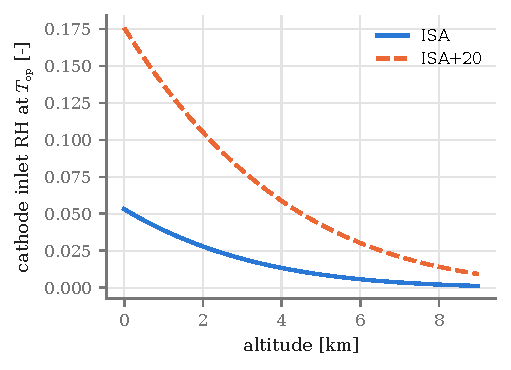
\includegraphics[width=0.55\textwidth]{figures/fig_humidity.pdf}
\caption{Cathode inlet relative humidity (at $T_\mathrm{op}=\SI{80}{\celsius}$, $p_c=\SI{1.5}{bar}$)
carried by saturated ambient air through the compressor, against altitude, from
\fn{FuelCell.cathode_inlet_rh}.}
\label{fig:humidity}
\end{figure}

\begin{table}[ht]
\centering\small
\caption{Weather and humidifier study on the reference design. Changes are relative to the dry
ISA day. Inlet RH and $x_v$ are at the take-off point.}
\label{tab:weather}
\setlength{\tabcolsep}{4pt}
\begin{tabular}{@{}lrrrrrr@{}}
\toprule
Case & $W_\mathrm{TO}$ [kg] & change & H$_2$ & take-off heat & TMS & inlet RH, $x_v$ \\
\midrule
ISA, dry & 21634 & -- & -- & -- & -- & 0.00, 1 \\
ISA, saturated & 21635 & +0.005\,\% & +0.01\,\% & +0.03\,\% & +0.03\,\% & 0.05, 1 \\
ISA+20, dry & 21726 & +0.42\,\% & +1.9\,\% & +1.9\,\% & +2.4\,\% & 0.00, 1 \\
ISA+20, saturated & 21730 & +0.44\,\% & +2.0\,\% & +2.0\,\% & +2.6\,\% & 0.17, 1 \\
ISA, humidifier $\phi_\mathrm{hum}=1$ & 22662 & +4.75\,\% & +2.5\,\% & +39.9\,\% & +37.2\,\% & 1.00, 0 \\
\bottomrule
\end{tabular}
\end{table}

Three results follow. First, ambient humidity is negligible: it changes $W_\mathrm{TO}$ by at most
\SI{0.02}{\percent} (ISA+20, saturated against dry), and $x_v$ stays 1. Second, the hot day costs
\SI{0.42}{\percent} of $W_\mathrm{TO}$, through the flight performance and the compressor work.
Third, a humidifier that saturates the inlet leaves no room in the exhaust for the product
water: $x_v=0$, all the latent heat goes to the coolant, the take-off heat grows by
\SI{40}{\percent}, the Class-I TMS by \SI{37}{\percent} and $W_\mathrm{TO}$ by \SI{4.75}{\percent}.
The model does not credit the humidifier with any benefit to the polarization curve, so this
case shows the heat penalty only.

\begin{figure}[ht]
\centering
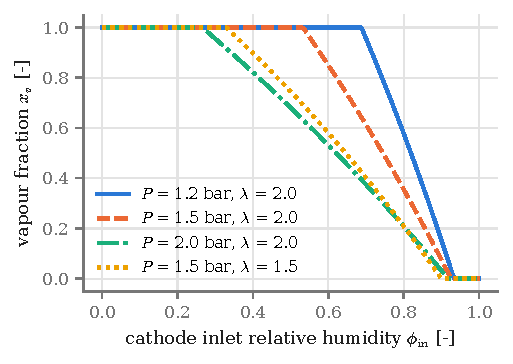
\includegraphics[width=0.55\textwidth]{figures/fig_vapour_fraction.pdf}
\caption{Product-water vapour fraction $x_v$ against the cathode inlet relative humidity, for
the \code{PEMFC_GoodPerformance} stack temperature (\SI{80}{\celsius}), from
\fn{FuelCell.product_water_vapour_fraction}.}
\label{fig:vapour}
\end{figure}

\paragraph{Heat per unit electrical power.} Combining Eqs.~\eqref{eq:pnet}--\eqref{eq:qcool},
the heat per unit gross power is $(V_\mathrm{tn}-V_\mathrm{cell})/V_\mathrm{cell}$, with
$V_\mathrm{tn}$ the thermoneutral voltage of Eq.~\eqref{eq:qcool}. The hydrogen per unit gross
power is proportional to $1/V_\mathrm{cell}$. A drop of the cell voltage, by load or by
degradation, therefore raises the heat much faster than the hydrogen. This ratio governs the
TMS sizing and the degradation results of Section~\ref{sec:degradation}.

%% =====================================================================================
\section{Stack design}
\label{sec:design}

This section describes how the stack is sized for a required propulsive power. One kernel,
\fn{FuelCell._size_stack(P_propulsive_design)} (\fn{FuelCell.py}, lines 467--554), sets the
cell geometry, the rated power and all the fuel-cell system masses. Two public methods call
it: \fn{SizeForPropulsivePower} and \fn{SizeFromConstraint} (Section~\ref{sec:closure}).

\subsection{The sizing kernel step by step}

\paragraph{First, the design current density.} The design current density $\jdes$ is the
point of the polarization curve, at the present state of health, where the cell voltage equals
the design cell voltage $\Vdes$ (\code{v_cell_design}):
\begin{equation}
  V_\mathrm{cell}(\jdes) = \Vdes, \qquad \jdes\in[10^{-4},\,5]\ \si{A/cm^2},
\end{equation}
solved with \fn{scipy.optimize.brentq}. If the bracket does not contain a root, the code
falls back to $\Vdes := V_\mathrm{cell}(i_\mathrm{rated})$ with $i_\mathrm{rated}$ the input
\code{i_rated}. The fallback is reached only for $\Vdes$ above $V_\mathrm{cell}(10^{-4})$,
about \SI{1.02}{V} for the database models (Table~\ref{tab:db}). For any practical design
voltage the input \code{i_rated} therefore has no effect: the attribute
\code{i_max_density} that stores it is overwritten by $\jdes$.

\paragraph{Second, the rated electrical power.} The required propulsive (thrust) power
$P_\mathrm{prop,des}$ is referred to the net stack terminals through the downstream chain:
\begin{equation}
  P_\mathrm{fc,rated} = \frac{P_\mathrm{prop,des}}{\eta_\mathrm{EM}\,\eta_\mathrm{PM}\,\eta_\mathrm{GB}\,\eta_\mathrm{prop}}
  + P_\mathrm{aux,TMS},
  \label{eq:prated}
\end{equation}
with the motor, PMAD, gearbox and propeller efficiencies from \code{EnergyInput} and
$P_\mathrm{aux,TMS}$ the coolant-pump power of a Class-II TMS (zero for Class I). The same
chain converts the demand at every mission point (Section~\ref{sec:operating}), so the rating
and the flown mission are consistent.

\paragraph{Third, the cell count.} The number of cells follows from the nominal bus voltage
$V_\mathrm{stack}$ (\code{stack_design_voltage}, default \SI{1000}{V}):
\begin{equation}
  N_\mathrm{cells} = \max\big(\lfloor V_\mathrm{stack}/\Vdes \rfloor,\ 100\big).
\end{equation}
The product $N_\mathrm{cells}A_\mathrm{cell}$ is fixed by the next step, and every flow, power
and heat depends on that product only. Therefore $V_\mathrm{stack}$ changes the cell count and
the cell area, but no mass and no mission result.

\paragraph{Fourth, the active area.} The total active area delivers the net rating at
$\jdes$ after an allowance for the parasitic loads:
\begin{equation}
  A_\mathrm{tot} = N_\mathrm{cells}A_\mathrm{cell}
  = \frac{P_\mathrm{fc,rated}/\eta_\mathrm{BoP,s}}{\Vdes\,\jdes}, \qquad
  \eta_\mathrm{BoP,s} = 0.85 .
  \label{eq:area}
\end{equation}
The constant $\eta_\mathrm{BoP,s}$ (\code{BoP_Power_Sizing_Efficiency}) is the fraction of the
gross power left after the air system and the fixed auxiliaries at the sizing point. The code
comment motivates the value: the measured parasitic draw is about \SI{4}{\percent} of gross at
sea level and about \SI{12}{\percent} at cruise altitude, and 0.85 covers the worst case with
a small margin. Figure~\ref{fig:efficiency}(b) confirms the order of magnitude for the
reference stack.

\paragraph{Fifth, the stack mass.} The input stack specific power $SP_\mathrm{stack}$
(\code{stack_power_density}, W/kg) is a hardware figure referenced to a cell voltage of
\SI{0.7}{V} on the beginning-of-life curve. The mass per unit active area is
\begin{equation}
  \frac{m_\mathrm{stack}}{A_\mathrm{tot}} = \frac{0.7\,j_\mathrm{ref}}{SP_\mathrm{stack}},
  \qquad V^\mathrm{BOL}_\mathrm{cell}(j_\mathrm{ref}) = \SI{0.7}{V},
  \label{eq:mstack}
\end{equation}
with $j_\mathrm{ref}=\SI{1.0}{A/cm^2}$ as a fallback if the root is not bracketed. The
reference is the BOL curve (\code{PolarizationCurve(..., bol=True)}), so a stack sized at end
of life is larger, not lighter (Section~\ref{sec:degradation}). A stack operated at a design
voltage below \SI{0.7}{V} delivers more power per kilogram than $SP_\mathrm{stack}$. For
\code{PEMFC_GoodPerformance}, $j_\mathrm{ref}=\SI{0.421}{A/cm^2}$ and the power density at
\SI{0.5}{V} is \SI{0.574}{W/cm^2} against \SI{0.295}{W/cm^2} at \SI{0.7}{V}, a ratio of 1.95.

\paragraph{Sixth, the balance of plant and the electric drive.}
\begin{gather}
  m_\mathrm{BoP} = r_\mathrm{BoP}\, m_\mathrm{stack}, \qquad
  m_\mathrm{EM} = \frac{P_\mathrm{drive}\,\eta_\mathrm{PM}}{SP_\mathrm{EM}}, \qquad
  m_\mathrm{PM} = \frac{P_\mathrm{drive}+P_\mathrm{aux,TMS}}{SP_\mathrm{PMAD}}, \nonumber\\
  P_\mathrm{drive} = \frac{P_\mathrm{prop,drive}}{\eta_\mathrm{EM}\,\eta_\mathrm{PM}\,\eta_\mathrm{GB}\,\eta_\mathrm{prop}},
  \label{eq:drive}
\end{gather}
with $r_\mathrm{BoP}$ the input \code{bop_mass_ratio}, $SP_\mathrm{EM}$ the second entry of
\code{specific_power_powertrain} (fallback \SI{5000}{W/kg}) and $SP_\mathrm{PMAD}$ from
\fn{Powertrain.pmad_specific_power} (fallback \SI{10000}{W/kg}). The motor carries the power
downstream of the PMAD and the PMAD the electrical drive power plus the pump. In
\code{'Hydrogen'} the drive power is the stack's propulsive design power,
$P_\mathrm{prop,drive}=P_\mathrm{prop,des}$, so the PMAD carries the full net rating
$P_\mathrm{fc,rated}$. In \code{'FuelCellBattery'} the battery feeds the same PMAD and motor,
so the drive is sized on the peak propulsive power through it at one instant, fuel-cell and
battery shares together:
\begin{equation}
  P_\mathrm{prop,drive} = \max\big(P_\mathrm{prop,des},\ \mathtt{SizingMargin}\cdot\mathtt{mission.Max\_PDrive}\big).
\end{equation}
\code{Max_PDrive} is the largest of the mission peak, the take-off/OEI requirement
$P_\mathrm{TO/OEI}$ and the ground-segment powers of the last flown mission
(Section~\ref{sec:fcb}). It is never below the fuel-cell share, so a design with $\varphi=0$
keeps the drive of the \code{'Hydrogen'} design. The fuel-cell system mass is
$m_\mathrm{FCS}=m_\mathrm{stack}+m_\mathrm{BoP}+m_\mathrm{EM}+m_\mathrm{PM}$. The kernel
writes it to \code{weight.WPT}; it also writes \code{weight.WThermal} $=m_\mathrm{stack}+m_\mathrm{BoP}+m_\mathrm{PM}$
and \code{weight.WElectric} $=m_\mathrm{EM}$ (the names are inherited from the gas-turbine
hybrid). Finally the kernel sets \code{Sizing_Done} and resets the adequacy trackers
(Section~\ref{sec:adequacy}).

\paragraph{Sizing margin.} \code{FuelCell.SizingMargin} (class attribute, default 1.0)
multiplies the required propulsive power in \fn{SizeForPropulsivePower}. It is the only
explicit power margin. The conservative case comes from the take-off and one-engine-inoperative
(OEI) requirements that the weight loop passes in, not from hidden factors.

\subsection{Reference design}
\label{sec:refdesign}

Throughout this manual the \emph{reference design} is
\fn{examples/common.py:hydrogen_config()}: an ATR~42-like aircraft (750~nm mission,
220~nm diversion, \SI{4560}{kg} payload), Class-I weight, \code{PEMFC_GoodPerformance},
$\Vdes=\SI{0.5}{V}$, $SP_\mathrm{stack}=\SI{2000}{W/kg}$, $r_\mathrm{BoP}=0.40$,
$\eta_\mathrm{EM}=0.96$, $\eta_\mathrm{PM}=0.99$, $\eta_\mathrm{GB}=0.96$,
$\eta_\mathrm{prop}=0.85$, $SP_\mathrm{EM}=SP_\mathrm{PMAD}=\SI{10000}{W/kg}$, Class-I TMS
with the default \SI{5000}{W/kg}, and the gravimetric-index tank with index 0.35. Sizing it
takes about \SI{15}{s}. Table~\ref{tab:refdesign} gives the stack it produces.

\begin{table}[ht]
\centering\small
\caption{Fuel-cell system of the reference design (\fn{make_figures.py:group_reference}).}
\label{tab:refdesign}
\begin{tabular}{@{}lr@{\hspace{2.5em}}lr@{}}
\toprule
Quantity & Value & Quantity & Value \\
\midrule
sizing propulsive power & \SI{2.989}{MW} & stack mass $m_\mathrm{stack}$ & \SI{1166}{kg} \\
downstream efficiency & 0.7755 & BoP mass $m_\mathrm{BoP}$ & \SI{466}{kg} \\
rated net power $P_\mathrm{fc,rated}$ & \SI{3.855}{MW} & motor mass $m_\mathrm{EM}$ & \SI{382}{kg} \\
design current density $\jdes$ & \SI{1.147}{A/cm^2} & PMAD mass $m_\mathrm{PM}$ & \SI{385}{kg} \\
$N_\mathrm{cells}$ & 2000 & fuel-cell system $m_\mathrm{FCS}$ & \SI{2400}{kg} \\
cell area $A_\mathrm{cell}$ & \SI{3954}{cm^2} & mass per active area & \SI{1.475}{kg/m^2} \\
total active area & \SI{791}{m^2} & $j_\mathrm{ref}$ at \SI{0.7}{V} & \SI{0.421}{A/cm^2} \\
\bottomrule
\end{tabular}
\end{table}

\subsection{The design-voltage trade}
\label{sec:vsweep}

The design cell voltage is the main stack design variable. A higher $\Vdes$ moves the design
point to a lower current density on the polarization curve. The cell is then more efficient,
but each square centimetre delivers less power, so the active area and the stack mass grow.
Example~21 (\fn{examples/21_hydrogen_design_voltage_sweep.py}) shows this trade. We repeat it
on the reference design from 0.40 to \SI{0.65}{V} (Figure~\ref{fig:vsweep},
\fn{make_figures.py:group_sweep}).

\begin{figure}[ht]
\centering
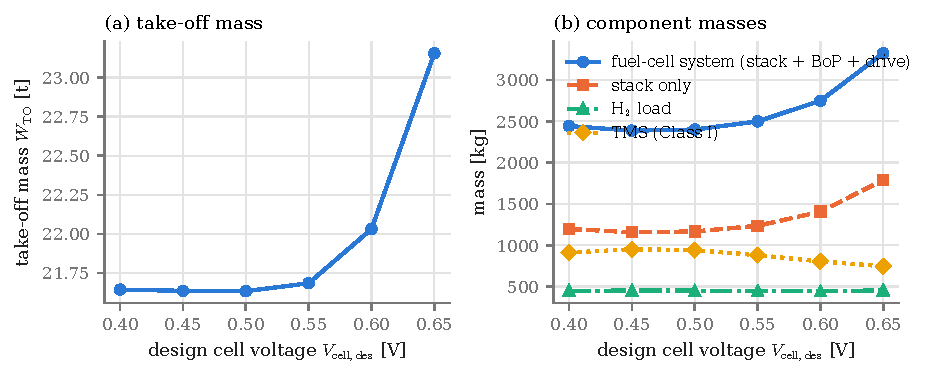
\includegraphics[width=\textwidth]{figures/fig_voltage_sweep.pdf}
\caption{Design-voltage sweep of the reference design: take-off mass (a) and component
masses (b). Each point is a full design with the weight loop closed.}
\label{fig:vsweep}
\end{figure}

The results have three features.
\begin{itemize}
  \item Between 0.40 and \SI{0.55}{V} the take-off mass is flat: \SI{21645}{kg},
  \SI{21637}{kg}, \SI{21634}{kg} and \SI{21685}{kg}. Above it the mass rises to
  \SI{22032}{kg} at \SI{0.60}{V} and \SI{23154}{kg} at \SI{0.65}{V}, where the stack mass is
  \SI{1787}{kg} against \SI{1166}{kg} at \SI{0.5}{V}.
  \item The hydrogen load changes little, from \SI{443}{kg} to \SI{453}{kg}. The stack is sized
  for the climb peak and runs well below its design current over most of the mission
  (Section~\ref{sec:history}), so the flown cell voltage depends weakly on $\Vdes$.
  \item Below the voltage of maximum power density (\SI{0.466}{V} for this model) a lower
  $\Vdes$ needs \emph{more} area, not less: \SI{811}{m^2} at \SI{0.40}{V} against
  \SI{791}{m^2} at \SI{0.50}{V}. Such designs are both less efficient and larger. A design
  voltage below the maximum-power-density point is therefore dominated.
\end{itemize}
The Class-I TMS mass falls with $\Vdes$ (\SI{909}{kg} at \SI{0.40}{V}, \SI{745}{kg} at
\SI{0.65}{V}), because a higher cell voltage rejects less heat per unit power
(Section~\ref{sec:heat}). This partly offsets the stack growth.

%% =====================================================================================
\section{Operating point}
\label{sec:operating}

This section describes how the code finds the stack state at one flight condition. The method
is \fn{FuelCell.ComputePRatio(alt, vel, P_req_net)} (\fn{FuelCell.py}, lines 632--740). The
mission calls it at every right-hand-side evaluation of the ODE integrator, so it is the most
frequently executed part of the model.

\subsection{From propulsive demand to electrical demand}

The argument \code{P_req_net} is the propulsive (thrust) power $P_\mathrm{prop}$ the fuel
cell must supply. The method first forms the downstream efficiency
\begin{equation}
  \eta_\mathrm{mech} = \eta_\mathrm{GB}\,\eta_\mathrm{EM}\,\eta_\mathrm{PM}\,\eta_\mathrm{prop},
\end{equation}
with the motor and propeller efficiencies from \fn{FuelCell.drive_efficiencies(alt, vel,
P_propulsive)}. Both are constants by default (\code{Eta Electric Motor}, \code{Eta
Propulsive}). When the powertrain has the Hamilton propeller attached, the propeller
efficiency is the powertrain's \code{'propeller'} model (\fn{Powertrain.eta}, wrapping
\fn{HamiltonPropellerEfficiency}, bounded to $[0.4,\,1]$), the same model the gas-turbine
graphs use. It is evaluated at its own shaft input $P_\mathrm{prop}/\eta_\mathrm{prop}$, a
fixed point started at $P_\mathrm{prop}$ (shaft-power tolerance $10^{-6}P_\mathrm{prop}$, at
most 50 iterations). The step is halved whenever it changes sign, because at low power the
propeller efficiency rises steeply with the shaft power and the plain iteration oscillates. When
\code{'Eta Electric Motor Model'} is \code{'Smart'}, the motor efficiency is the operating-point
value of the Class-II d-q motor model (\fn{Powertrain.eta} for the component
\code{'electric_motor'}, wrapping \fn{Systems/Powertrain/efficiency.py:MotorEfficiencyModel};
see example~25), evaluated at its shaft output $P_\mathrm{prop}/(\eta_\mathrm{GB}\eta_\mathrm{prop})$.
In \code{'FuelCellBattery'} each branch evaluates these models at its own share of the
propulsive power, although the two branches share the motor and the propeller; this is an
approximation that does not affect constant efficiencies. The electrical target is
\begin{equation}
  \Pel = \frac{P_\mathrm{prop}}{\max(\eta_\mathrm{mech},0.01)} + P_\mathrm{aux,TMS}.
\end{equation}

\subsection{The root solve}

The residual is the net power of Eq.~\eqref{eq:pnet} minus the target,
\begin{equation}
  \mathcal R(j) = P_\mathrm{net}(j;\,h) - \Pel ,
\end{equation}
set to $-2\Pel$ when $V_\mathrm{cell}(j)\le\SI{0.1}{V}$. At fixed altitude, $P_\mathrm{net}(j)$
rises from $-P_\mathrm{fix}$ at zero current to a maximum and then falls, so the equation has
two roots when the demand is feasible. The code takes the lowest-current root, which lies on
the efficient branch:
\begin{enumerate}
  \item $\mathcal R$ is evaluated on a grid of 50 points from \SI{e-4}{A/cm^2} to
  $0.95\,j_\mathrm{lim}$.
  \item If the grid has a sign change, \fn{brentq} refines the first one (tolerance
  \SI{e-4}{A/cm^2}). This is the normal branch.
  \item If $\mathcal R\ge0$ already at the first grid point, that point is taken.
  \item Otherwise the maximum net power $P_\mathrm{net,max}$ is refined with a bounded scalar
  minimisation around the best grid point. If $P_\mathrm{net,max}\le0$ the method raises
  \code{FuelCellError(code="FC_NO_NET_POWER")}. If $P_\mathrm{net,max}\ge\Pel$ the root lies
  between two grid points and is found with \fn{brentq}. Otherwise the stack is
  \emph{power-limited} (next subsection).
\end{enumerate}

\subsection{The power-limited branch}
\label{sec:powerlimited}

When the demand exceeds the maximum net power, the stack runs at its maximum-net-power current
density $j_\mathrm{mp}$ and the shortfall is supplied at that point's efficiency. The code
introduces the scale factor
\begin{equation}
  s = \frac{\Pel}{P_\mathrm{net,max}} > 1
\end{equation}
and multiplies the gross power, the air-system powers, the hydrogen flow, the air flow and the
heat by $s$. The flows and the heat are therefore those of a stack $s$ times larger running at
$j_\mathrm{mp}$. On the feasible branch $s=1$. The branch is continuous with the feasible one
at $s=1$, and the hydrogen and the heat keep growing with the demand and with the degradation.
The point is flagged in
\code{_power_limited}, so the mission closes but the design is reported as infeasible.

Figure~\ref{fig:powerlimited} shows the branch on the reference stack at sea level and
\SI{70}{m/s}. The maximum propulsive power the BOL stack delivers there is \SI{3.40}{MW}. The
hydrogen flow and the heat cross the limit without a jump. With a uniform loss of
\SI{50}{mV} the limit moves down to about 0.895 of the BOL limit (resolution of the sweep:
0.005), and at \SI{1.2}{} times the
BOL limit the hydrogen flow is \SI{132.9}{g/s} against \SI{122.3}{g/s} at BOL, while the heat is
\SI{10.42}{MW} against \SI{9.17}{MW}.

\begin{figure}[ht]
\centering
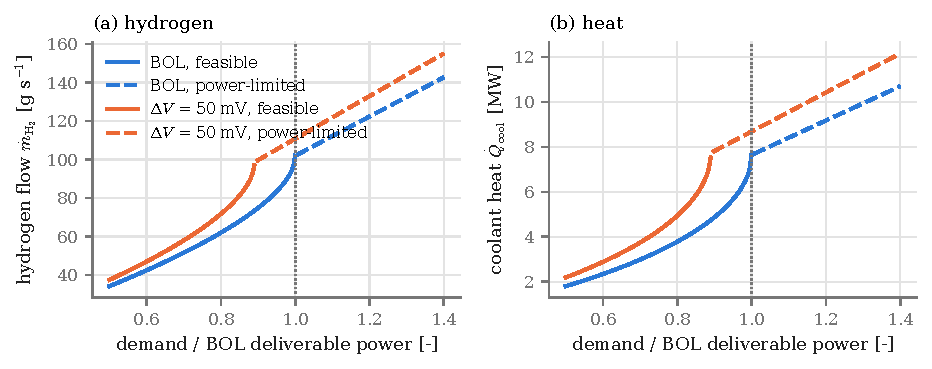
\includegraphics[width=\textwidth]{figures/fig_power_limited.pdf}
\caption{Hydrogen flow (a) and coolant heat (b) of the reference stack at sea level against
the propulsive demand, normalised by the BOL deliverable power. Solid: feasible branch; dashed:
power-limited branch ($s>1$).}
\label{fig:powerlimited}
\end{figure}

\subsection{Outputs}

After the solve the method stores the operating point:
$j$ (\code{i_op_last}), $V_\mathrm{cell}$ (\code{v_cell_last}), $\eta_\mathrm{FCS}$
(\code{eta_fcs_last}), $s\,P_\mathrm{gross}$ (\code{P_gross_last}),
$s\,P_\mathrm{comp,net}$ (\code{P_comp_net_last}), $s\,P_\mathrm{turb}$
(\code{P_turb_last}), $\dot m_{\mathrm{H_2}}$ (\code{mdot_h2}), $\dot m_\mathrm{air}$
(\code{mdot_air}), $x_v$ (\code{x_vapour}) and $\dot Q_\mathrm{cool}$ (\code{Q_thermal}).
Here $\eta_\mathrm{FCS}=\Pel/P_\mathrm{chem}$, with the scaled chemical power. The method also
returns the two-element array \code{[1/eta_total, 1.0]} with
\begin{equation}
  \eta_\mathrm{total} = \operatorname{clip}\!\left(\eta_\mathrm{FCS}\,\eta_\mathrm{mech}\,
  \frac{P_\mathrm{prop}/\eta_\mathrm{mech}}{\Pel},\ 0.01,\ 0.85\right).
\end{equation}
No quantity of the package is computed from this ratio, and the clip has no effect on any
result. The mission charges hydrogen with the stack's own hydrogen flow,
$P_\mathrm{chem}=\dot m_{\mathrm{H_2}}\,\mathrm{HHV}$ (Section~\ref{sec:mission}), which has no
clipping and is not zero at zero propulsive power. The take-off hydrogen power
\code{mission.TO_P_H2_Thermal} is the same quantity at the take-off point. Without the clip
the ratio times $P_\mathrm{prop}$ equals $P_\mathrm{chem}$, so the two differ only where the
clip is active.

\subsection{Efficiency and heat versus load}
\label{sec:effload}

Figure~\ref{fig:efficiency} sweeps the reference stack (sized as in
Table~\ref{tab:refdesign}) over the electrical load $\Pel/P_\mathrm{fc,rated}$ at four
altitudes and \SI{120}{m/s}. The net efficiency peaks at a load of about 0.2: 0.484 at sea level
and 0.460 at \SI{8}{km}. At lower loads the constant fixed auxiliary load
($0.015\,P_\mathrm{fc,rated}$) dominates; at higher loads the cell voltage falls. At full load
the efficiency is 0.378 at sea level and 0.330 at \SI{8}{km}. The net air-system power at full
load rises from \SI{2.5}{\percent} of the gross power at sea level to \SI{9.2}{\percent} at
\SI{8}{km}. The highest feasible load falls with altitude, from 1.13 at sea level to 1.05 at
\SI{8}{km}. This is why the sizing allowance $\eta_\mathrm{BoP,s}=0.85$ is needed.

\begin{figure}[ht]
\centering
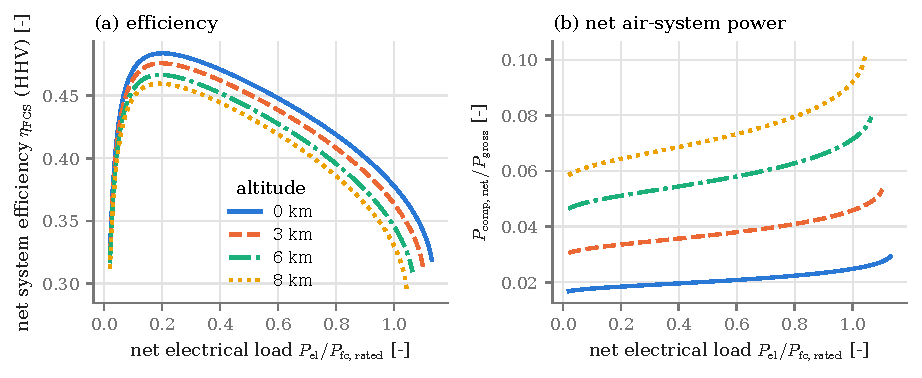
\includegraphics[width=\textwidth]{figures/fig_efficiency_load.pdf}
\caption{Reference stack: net system efficiency on the HHV basis (a) and net air-system power
as a fraction of the gross power (b) against the net electrical load, at four altitudes.
Curves end at the power limit.}
\label{fig:efficiency}
\end{figure}

Figure~\ref{fig:heatload} gives the coolant heat per unit net electrical power. With vapour
product water ($x_v=1$, the computed value) it is 0.63 at a load of 0.1 and 1.20 at full load at
sea level; at \SI{8}{km} the full-load value is 1.44. With liquid product water ($x_v=0$) the
same quantities are 0.96, 1.63 and 2.11. At full load the stack therefore rejects more heat than
it delivers electrical power.

\begin{figure}[ht]
\centering
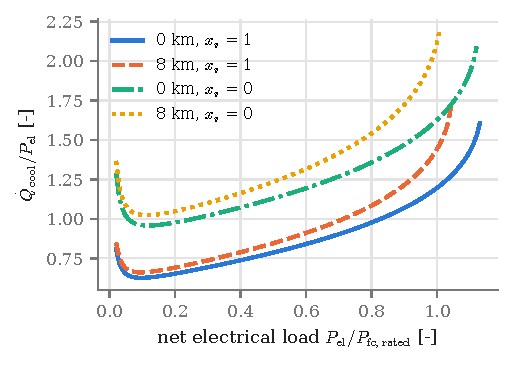
\includegraphics[width=0.55\textwidth]{figures/fig_heat_load.pdf}
\caption{Reference stack: coolant heat per unit net electrical power against load, at sea
level and \SI{8}{km}, for vapour ($x_v=1$) and liquid ($x_v=0$) product water.}
\label{fig:heatload}
\end{figure}

\subsection{Adequacy tracking and \texttt{report\_sizing}}
\label{sec:adequacy}

At every call \fn{ComputePRatio} records the load ratio $\Pel/P_\mathrm{net,max}$, keeps the
worst one (\code{_worst_load_ratio}) with its altitude and demand, and sets
\code{_power_limited} when the ratio exceeds $1+10^{-6}$. The trackers are reset by
\fn{_size_stack} and by \fn{reset_adequacy}, so they always describe the last stack and the
last mission flown. \fn{FuelCell.report_sizing(raise_on_undersize=False)} turns them into a
dictionary with keys \code{rated_power}, \code{worst_load_ratio}, \code{worst_altitude},
\code{peak_demand}, \code{power_limited}, \code{min_rating} and \code{status}. The status is
\code{'UNDERSIZED'} when power-limited, \code{'oversized'} when the worst ratio is below 0.5,
\code{'ok'} otherwise, and \code{'unknown'} before any mission. An undersized stack triggers a
warning (or a \code{ValueError} with \code{raise_on_undersize=True}).
\fn{Aircraft.DesignAircraft} calls \fn{report_sizing} at the end of every fuel-cell design.
For the reference design the worst load ratio is 0.890, at \SI{2597}{m} in the second climb
segment, and the status is \code{'ok'}.

%% =====================================================================================
\section{Mission and weight closure}
\label{sec:closure}

This section describes how the fuel cell is flown over the mission and closed with the
take-off weight. The point is that the stack that flies the mission is the stack that is
weighed, and that the take-off and OEI requirements are a hard floor on its rating.

\subsection{Mission integration}
\label{sec:mission}

\fn{Mission.HydrogenConfiguration(WTO)} integrates two states over the mission and diversion:
the cumulative hydrogen chemical energy $E$ and the mass fraction $\beta=W/W_\mathrm{TO}$,
\begin{equation}
  \frac{dE}{dt} = \dot m_{\mathrm{H_2}}\big(P_\mathrm{prop}(\beta,t)\big)\,\mathrm{HHV}, \qquad
  \frac{d\beta}{dt} = -\frac{dE/dt}{e_f\,W_\mathrm{TO}} ,
  \label{eq:missionode}
\end{equation}
with $P_\mathrm{prop}=W_\mathrm{TO}\cdot$\fn{Performance.PoWTO}, clipped at zero by
\fn{Mission.check_PP}, and $\dot m_{\mathrm{H_2}}$ the hydrogen flow that \fn{ComputePRatio}
leaves on the fuel cell (\fn{Mission._fuel_cell_chemical_power}). This flow also feeds the
air system, the fixed auxiliaries and a Class-II TMS pump, so the stack burns hydrogen even at
zero propulsive power. Each profile segment is integrated
separately with \code{solve_ivp} (BDF, \code{rtol=1e-5}, \code{max_step=60} s). The method
records the mission peak propulsive power (\code{Max_PEng}), the integrator solutions
(\code{integral_solution}) and the heat points for the TMS (next subsection). Before the
profile it evaluates the off-mission requirement
\begin{equation}
  P_\mathrm{TO/OEI} = \max\big(P_\mathrm{take\text{-}off},\, P_\mathrm{OEI\ climb}\big)
\end{equation}
at the constraint-diagram conditions (\fn{Mission._worst_case_propulsive_power}) and stores it
as \code{TO_PP}. These conditions are not flown by the profile, but the stack must supply them.

\paragraph{Heat points.} \fn{_takeoff_fc_heat} flies the stack once at $P_\mathrm{TO/OEI}$ at the
take-off altitude and speed, stores the heat as \code{TO_FC_Thermal_Pwr} and the hydrogen
chemical power of the stack, $\dot m_{\mathrm{H_2}}\,\mathrm{HHV}$, as \code{TO_P_H2_Thermal}
(both 0 when the battery supplies the whole take-off power), and starts the list
\code{mission.thermal_profile} with that point. After each segment is integrated,
\fn{_track_fc_heat_on_solution} re-evaluates the stack at the accepted solver points of the
segment (not at the trial evaluations inside the ODE right-hand side), and \fn{_track_fc_heat}
keeps the mission peak heat (\code{Max_FC_Thermal_Pwr}, with its altitude
and speed) and the peak of each segment, which \fn{_end_thermal_phase} appends to
\code{thermal_profile}. The Class-I TMS uses the largest of these heats; the Class-II TMS
chooses its design point among them (see \emph{PhlyGreen Technical Manual: Thermal
Management}).

\paragraph{Ground segments.} The flown profile starts at the beginning of the climb.
\fn{Mission._ground_segments} adds the taxi-out, the take-off run and the taxi-in. The take-off
run lasts \code{takeoff_time} (default \SI{0.7}{min}) at \code{takeoff_power_fraction}
(default 1.0) of the take-off-field propulsive power $P_\mathrm{take\text{-}off}$. Taxi-out and
taxi-in last \SI{13}{min} each at \code{taxi_power_fraction} (default 0.07) of it. These are
the ICAO LTO reference values cited in the code. For the fuel-cell configurations
\fn{_ground_power_split} evaluates \fn{ComputePRatio} at the take-off condition, so part-load
efficiency applies. The take-off battery share is the $\varphi$ of the profile's
\code{'Takeoff'} stage and the taxi share is \code{taxi_phi} (\code{'Taxi Supplied Power
Ratio'}), defaulting to the take-off share; both are zero for \code{'Hydrogen'}, and a non-zero
\code{taxi_phi} on a configuration without battery raises a \code{ValueError}. The taxi-out and
take-off hydrogen sets the mass fraction at the start of the climb,
$\beta_0 = 1 - E_\mathrm{out}/(e_f W_\mathrm{TO})$, and the ground energy is added to the
mission energy. For the reference design the taxi runs at \SI{0.048}{A/cm^2}
(\SI{4.2}{\percent} of $\jdes$) and \SI{0.831}{V}, the ground segments burn
\SI{1.267}{GJ} of hydrogen (\SI{8.9}{kg}) and $\beta_0=0.99973$.

\subsection{The self-consistent sizing loop}
\label{sec:loop}

\fn{Weight._fuel_cell_and_tms_closure(WTO)} sizes the fuel cell at one trial take-off weight.
It is shared by \fn{Weight.Hydrogen} and \fn{Weight.FuelCellBattery}.
\begin{enumerate}
  \item Reset the TMS couplings ($P_\mathrm{aux,TMS}=0$, \code{aerodynamics.extra_Cd} $=0$) and
  seed the stack with \fn{SizeFromConstraint(WTO)}. The seed power is
  $\max(\mathtt{DesignPW},\,\SI{155}{W/kg})$ times $W_\mathrm{TO}$, or times \SI{25000}{kg}
  when $W_\mathrm{TO}<\SI{10000}{kg}$. \code{DesignPW} is the constraint-diagram
  power-to-weight, which already contains the take-off and OEI requirements.
  \item Fly the mission (\fn{EvaluateMission}) and form the demand
  $P_\mathrm{req}=\max(\mathtt{TO\_PP},\,\mathtt{Max\_PEng})$.
  \item If $P_\mathrm{req}$ changed by less than $10^{-3}$ relative to the previous pass (and,
  with a Class-II TMS, the pump power and drag increment have settled), stop. Otherwise resize
  with \fn{SizeForPropulsivePower}$(P_\mathrm{req})$ and return to step 2.
\end{enumerate}
The loop runs at most three passes (\code{_FC_RESIZE_ITERS}), or six with a Class-II TMS
(\code{_FC_TMS_RESIZE_ITERS}). If it has not converged the mission is flown once more, so that
the energies returned always belong to the final stack. Within the loop $W_\mathrm{TO}$ is
fixed, so the propulsive power changes between passes only through the mass fraction $\beta$,
which depends weakly on the stack efficiency. This is why a few passes suffice.

\paragraph{Coupling with a Class-II TMS.} With \code{TMSConfig(tms_class='II')} each pass also
sizes the TMS on \code{mission.thermal_profile}. Two quantities feed back. The coolant-pump
power becomes the constant electrical load $P_\mathrm{aux,TMS}$, which enters
Eq.~\eqref{eq:prated} and every operating point. The ram-air duct drag becomes a drag-coefficient
increment \code{aerodynamics.extra_Cd}, referred to the wing area
$S=W_\mathrm{TO}g/(W/S)$. The loop then also waits for these two to converge. The physics of
the TMS is documented in \emph{PhlyGreen Technical Manual: Thermal Management}.

\paragraph{Reference design.} The take-off-field power is \SI{2.803}{MW} and the OEI climb
power \SI{2.393}{MW}, so \code{TO_PP} $=\SI{2.803}{MW}$. The mission peak is \SI{2.989}{MW}, in
the climb. The climb, not the take-off, sizes the stack.

\subsection{Take-off-weight equation}

\fn{Weight.Hydrogen} solves, with Brent's method (\fn{scipy.optimize.brenth} in
\fn{Weight._solve_wto}, with a grid-scan fallback) on $[1000,\,300000]$~kg,
\begin{equation}
  W_\mathrm{TO} = W_\mathrm{struct} + m_\mathrm{FCS} + W_{\mathrm{H_2}} + W_\mathrm{tank}
  + W_\mathrm{TMS} + W_\mathrm{payload} + W_\mathrm{crew} + W_\mathrm{reserve}.
\end{equation}
The terms are as follows.
\begin{itemize}
  \item $W_{\mathrm{H_2}} = (E/e_f)(1+m_{\mathrm{H_2}})$, with $E$ the mission plus ground
  hydrogen energy and $m_{\mathrm{H_2}}$ the input \code{h2_fuel_margin} (default 0.05) for
  unusable hydrogen and the feed system.
  \item $W_\mathrm{reserve}$ is \code{contingency_fuel} if given, else
  $0.05\,W_{\mathrm{H_2}}$, recomputed at every iteration.
  \item $W_\mathrm{tank}$ is the empty tank holding $W_{\mathrm{H_2}}+W_\mathrm{reserve}$
  (Section~\ref{sec:tank}).
  \item $W_\mathrm{TMS}$ is \fn{_fuel_cell_tms_mass}: for Class I the largest of the mission
  peak heat and the take-off heat divided by \code{hex_specific_power_h2} (default
  \SI{5000}{W/kg}); for Class II the mass of the sized TMS.
\end{itemize}
If no root is found the method raises a \code{RuntimeError} that suggests a lower design
voltage, a higher stack power density or a shorter mission. For the reference design the
breakdown is: structure \SI{11886}{kg}, fuel-cell system \SI{2400}{kg}, hydrogen
\SI{450}{kg}, reserve \SI{22}{kg}, tank \SI{877}{kg}, TMS \SI{940}{kg}, payload \SI{4560}{kg}
and crew \SI{500}{kg}, for $W_\mathrm{TO}=\SI{21634}{kg}$.

\subsection{Mission time histories}
\label{sec:history}

Figure~\ref{fig:history} shows the operating point along the reference mission and diversion,
re-evaluated on a \SI{5}{s} grid from the integrator solution
(\fn{make_figures.py:mission_history}). The current density never exceeds
\SI{0.88}{A/cm^2}, against $\jdes=\SI{1.147}{A/cm^2}$, and the cell voltage never falls below
\SI{0.580}{V}. The reason is the sizing allowance $\eta_\mathrm{BoP,s}=0.85$ of
Eq.~\eqref{eq:area}. At the climb peak (\SI{2597}{m}) the real parasitic draw is well below
\SI{15}{\percent} of the gross power (Figure~\ref{fig:efficiency}b), so the stack meets the
peak demand at a load ratio of 0.890 and a current density below $\jdes$. In cruise the
cell runs at \SI{0.34}{A/cm^2} and \SI{0.72}{V}, with $\eta_\mathrm{FCS}=0.439$. The heat peaks
at \SI{4.70}{MW} in the climb (at \SI{1200}{m}), above the \SI{4.02}{MW} of the take-off point.
The propulsive power is positive everywhere on this profile, so the zero-power hydrogen of the
fixed auxiliaries plays no role here. The product water leaves fully as vapour ($x_v=1$) at every
point.

\begin{figure}[ht]
\centering
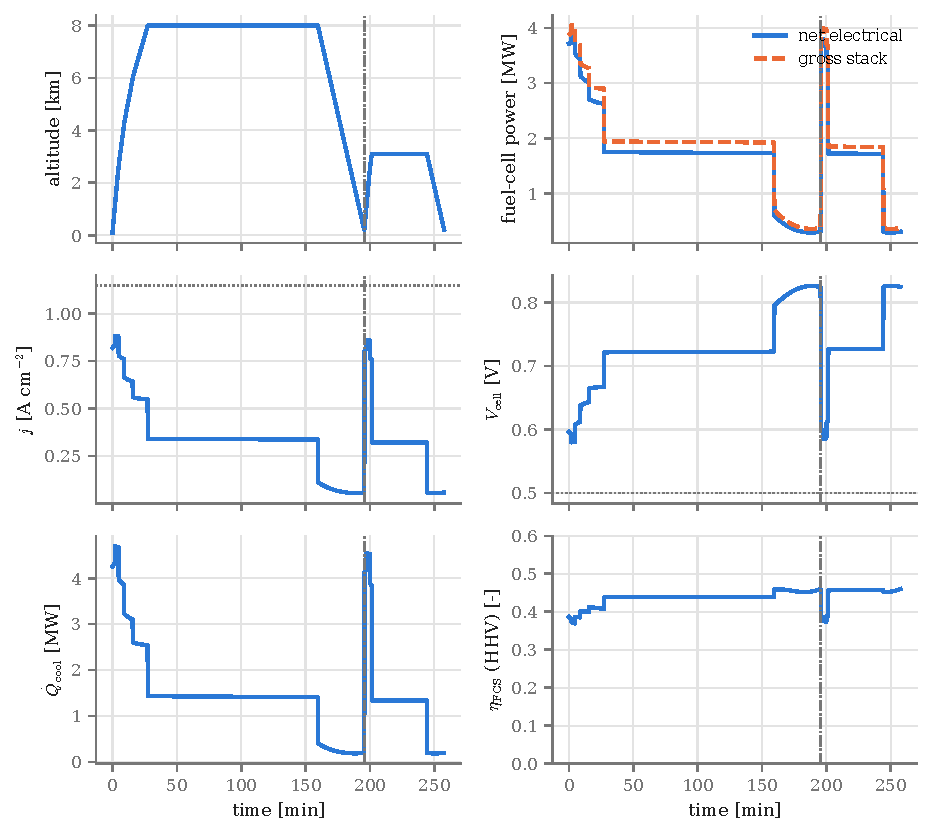
\includegraphics[width=\textwidth]{figures/fig_mission_history.pdf}
\caption{Reference design: altitude, fuel-cell power, current density, cell voltage, coolant
heat and net system efficiency along the mission and diversion. Dotted lines: design values
$\jdes$ and $\Vdes$. Dash-dotted line: end of the nominal mission.}
\label{fig:history}
\end{figure}

\subsection{Hydrogen storage}
\label{sec:tank}

The tank model is selected in \fn{Weight._hydrogen_tank_mass(m_h2, LH2_Tank, grav_index)}.
Without a \code{TankConfig}, or when CoolProp is not installed, the empty tank mass follows
from the gravimetric index $GI$ (\code{h2_gravimetric_index}, default 0.35), defined as
usable hydrogen over hydrogen plus tank:
\begin{equation}
  W_\mathrm{tank} = m_{\mathrm{H_2}}\left(\frac{1}{GI}-1\right).
\end{equation}
With a \code{TankConfig} the cryogenic \fn{Systems/Tank/Tank.py:LH2_Tank} is built for the
stored mass. It sizes the inner vessel and the vacuum jacket, and the multi-layer insulation,
after Svensson et al.~\cite{svensson} (\fn{TANK_Database.py}, model \code{'Svensson_Default'}).
Its transient method \fn{time_step} advances the tank state with heat leak, self-pressurisation,
venting at $P_\mathrm{max}$ and heating at $P_\mathrm{min}$. Setting
\code{mission.track_tank = True} and re-running \fn{EvaluateMission} drives it with the
hydrogen flow $\dot E/e_f$ of each integrator step and fills \code{aircraft.tank.history}
(example~22). The tank is a separate subsystem; we do not document it further here.

%% =====================================================================================
\section{Fuel cell + battery hybrid: the fuel-cell side}
\label{sec:fcb}

This section describes how the \code{'FuelCellBattery'} configuration loads and sizes the fuel
cell. The battery model, its sizing by energy and power, and its Class-II cell model are
documented in \emph{PhlyGreen Technical Manual: Battery}.

\subsection{Power split}

The profile supplies, at every instant, the battery fraction $\varphi(t)$ of the propulsive
power (\fn{profile.SuppliedPowerRatio}). In \fn{Mission.FuelCellBatteryConfiguration} the
fuel cell supplies
\begin{equation}
  P_\mathrm{prop,fc}(t) = \big(1-\varphi(t)\big)\,P_\mathrm{prop}(t),
\end{equation}
and its hydrogen follows from the stack flow exactly as in the pure-hydrogen mission
(Eq.~\eqref{eq:missionode}). The fuel cell is off only when $\varphi\ge1$; at any smaller
$\varphi$ it runs and burns hydrogen for its auxiliaries even at zero propulsive share. The ODE
has the same two states, so a design with $\varphi=0$ reproduces the \code{'Hydrogen'} design.
The battery energy is a passive integral computed after the integration, of the battery
\emph{terminal} power (\fn{Mission._fc_battery_terminal_power})
\begin{equation}
  P_\mathrm{bat} = \frac{\varphi P_\mathrm{prop}}{\eta_\mathrm{EM}\,\eta_\mathrm{PM}\,\eta_\mathrm{GB}\,\eta_\mathrm{prop}} ,
\end{equation}
with the same chain as the fuel-cell branch (\fn{Mission._fc_battery_eta_elec}, including a
propeller model or a Class-II motor model when selected). The battery peak powers
\code{Max_PBat} and \code{TO_PBat} are terminal powers too.
With a Class-II battery (\code{CellConfig(cell_class='II')})
\fn{FuelCellBatteryConfigurationClassII} applies the same split and integrates the cell
model with the P-number sizing of the pack.

The take-off and OEI requirement is split by the take-off share $\varphi_\mathrm{TO}$, the
$\varphi$ of the profile's \code{'Takeoff'} stage:
\begin{equation}
  \mathtt{TO\_PP} = (1-\varphi_\mathrm{TO})\,P_\mathrm{TO/OEI}, \qquad
  \mathtt{TO\_PBat} = \frac{\varphi_\mathrm{TO}\,P_\mathrm{TO/OEI}}
  {\eta_\mathrm{EM}\eta_\mathrm{PM}\eta_\mathrm{GB}\eta_\mathrm{prop}},
\end{equation}
the second evaluated at the take-off altitude and true airspeed of
\fn{Mission._ground_condition}.
The battery is therefore assumed to assist the OEI climb with the same share as the take-off
run. The fuel cell is sized by the loop of Section~\ref{sec:loop} on
\begin{equation}
  P_\mathrm{req} = \max\!\Big((1-\varphi_\mathrm{TO})\,P_\mathrm{TO/OEI},\ \max_t\,(1-\varphi)P_\mathrm{prop}\Big).
  \label{eq:fcbreq}
\end{equation}
A larger $\varphi$ shrinks the stack, but only until the other term of Eq.~\eqref{eq:fcbreq}
takes over.

\paragraph{Ground segments.} The battery also carries a share of the ground power
(\fn{Mission._ground_power_split}): $\varphi_\mathrm{TO}$ of the take-off run and
\code{taxi_phi} of the taxi power, with \code{taxi_phi} defaulting to $\varphi_\mathrm{TO}$.
The fuel cell supplies the rest. The battery terminal energy of these legs is added to the
battery energy, and their terminal powers to \code{Max_PBat}, so a battery that assists the
take-off also covers $\varphi_\mathrm{TO}$ of the 26 minutes of taxi unless \code{taxi_phi} is
set to zero.

\paragraph{Drive sizing.} The battery feeds the same PMAD and motor as the stack. The mission
therefore records \code{Max_PDrive}, the largest propulsive power through the drive at one
instant with both shares together: the mission peak of $P_\mathrm{prop}$, the take-off/OEI
requirement $P_\mathrm{TO/OEI}$ and, added by \fn{EvaluateMission}, the take-off-run and taxi
powers. The kernel sizes the motor and the PMAD on it (Eq.~\eqref{eq:drive}). A battery share
therefore shrinks the stack, its balance of plant and the TMS, but not the motor and the PMAD,
which still carry the full take-off power and change only with $W_\mathrm{TO}$.

\subsection{When does a take-off battery pay?}

Example~23 (\fn{examples/23_fuelcell_battery_hybrid.py}) studies when a battery makes a
fuel-cell aircraft lighter. A battery pays only if it lowers the power that sizes the fuel cell
by more than its own mass, and the snowball of that mass, costs. The example varies one lever for
each of the two conditions this implies: the take-off field, which decides whether the take-off
sizes the fuel cell, and the battery specific power, which decides how much the battery weighs
per kilowatt. Its take-off-assist strategy puts the battery on the take-off run only:
$\varphi_\mathrm{TO}$ on the \code{'Takeoff'} stage, $\varphi=0$ in flight and
\code{taxi_phi = 0}. The configuration is \fn{common.fuelcell_battery_config(cruise_phi=0.0)}
with a Class-I battery (\SI{250}{Wh/kg}, usable SOC 0.8). The two fields are the baseline
\SI{1107}{m} and the \SI{800}{m} runway of the ATR~42-600S short-field version. The two packs
are the default \SI{1.5}{kW/kg} pack of \fn{common.py} and a \SI{3}{kW/kg} power pack. The
\SI{3}{kW/kg} value, and the higher values of the specific-power scan below, are assumed
technology levels for the study, not sourced pack data. \fn{make_figures.py:group_assist} runs
the example's own \fn{design} function and reproduces its output. Figure~\ref{fig:assist} and
Table~\ref{tab:assist} give the results.

\begin{figure}[ht]
\centering
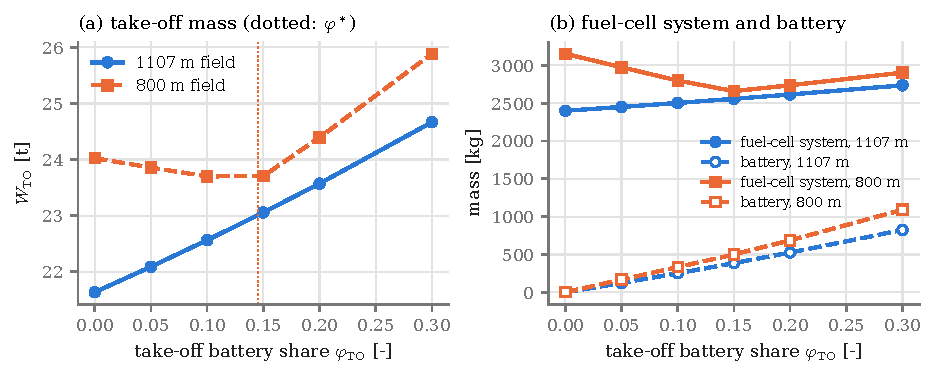
\includegraphics[width=\textwidth]{figures/fig_takeoff_assist.pdf}
\caption{Take-off assist of example~23 (battery on the take-off run only). (a) Change of the
take-off mass against the pure fuel-cell design ($\varphi_\mathrm{TO}=0$) for the two fields and
the two packs; the dotted line is $\varphi^*$ of Eq.~\eqref{eq:phistar} for the \SI{800}{m}
field. (b) The same change on the \SI{800}{m} field at $\varphi_\mathrm{TO}=0.15$ against the
battery specific power. Specific powers above \SI{1.5}{kW/kg} are assumed values.}
\label{fig:assist}
\end{figure}

\begin{table}[ht]
\centering\small
\caption{Take-off assist sweep of example~23 (\fn{make_figures.py:group_assist}): take-off
mass, fuel-cell system ($m_\mathrm{FCS}$: stack, BoP, PMAD and motor), battery, hydrogen load and
Class-I TMS, in kg.}
\label{tab:assist}
\setlength{\tabcolsep}{4pt}
\begin{tabular}{@{}lrrrrr@{\hspace{2em}}rrrrr@{}}
\toprule
 & \multicolumn{5}{c}{\SI{1.5}{kW/kg} pack (default)} & \multicolumn{5}{c@{}}{\SI{3}{kW/kg} power pack (assumed)} \\
\cmidrule(lr){2-6}\cmidrule(l){7-11}
field, $\varphi_\mathrm{TO}$ & $W_\mathrm{TO}$ & $m_\mathrm{FCS}$ & battery & H$_2$ & TMS
 & $W_\mathrm{TO}$ & $m_\mathrm{FCS}$ & battery & H$_2$ & TMS \\
\midrule
\SI{1107}{m}, 0.00 & 21634 & 2400 & 0 & 449.7 & 940 & 21634 & 2400 & 0 & 449.7 & 940 \\
\SI{1107}{m}, 0.05 & 22093 & 2451 & 123 & 459.0 & 960 & 21860 & 2425 & 61 & 454.2 & 949 \\
\SI{1107}{m}, 0.10 & 22570 & 2504 & 251 & 468.7 & 980 & 22090 & 2450 & 123 & 458.7 & 959 \\
\SI{1107}{m}, 0.15 & 23066 & 2559 & 385 & 478.8 & 1002 & 22326 & 2476 & 186 & 463.4 & 970 \\
\SI{1107}{m}, 0.20 & 23584 & 2616 & 525 & 489.4 & 1024 & 22565 & 2503 & 251 & 468.3 & 980 \\
\SI{1107}{m}, 0.30 & 24688 & 2739 & 825 & 511.9 & 1072 & 23060 & 2558 & 385 & 478.2 & 1002 \\
\midrule
\SI{800}{m}, 0.00 & 24024 & 3153 & 0 & 493.8 & 1213 & 24024 & 3153 & 0 & 493.8 & 1213 \\
\SI{800}{m}, 0.05 & 24067 & 3051 & 169 & 497.9 & 1155 & 23723 & 3008 & 83 & 490.8 & 1138 \\
\SI{800}{m}, 0.10 & 24119 & 2950 & 339 & 502.9 & 1096 & 23438 & 2867 & 165 & 488.7 & 1065 \\
\SI{800}{m}, 0.15 & 24321 & 2877 & 513 & 511.6 & 1068 & 23298 & 2756 & 246 & 490.1 & 1023 \\
\SI{800}{m}, 0.20 & 25046 & 2962 & 704 & 526.5 & 1100 & 23626 & 2794 & 332 & 496.7 & 1038 \\
\SI{800}{m}, 0.30 & 26627 & 3149 & 1123 & 559.1 & 1170 & 24310 & 2875 & 513 & 510.5 & 1068 \\
\bottomrule
\end{tabular}
\end{table}

\paragraph{The take-off must size the fuel cell.} On the \SI{1107}{m} field the climb peak
(\SI{2989}{kW}) exceeds the take-off propulsive power (\SI{2803}{kW}). The take-off battery
removes no stack mass, and every share makes the aircraft heavier with either pack. On the
\SI{800}{m} field the take-off needs \SI{3928}{kW} against \SI{3357}{kW} for the climb, so the
take-off sizes the stack. The battery removes stack mass until it brings the fuel cell's
take-off load down to its climb load, at the share
\begin{equation}
  \varphi^* = 1 - \frac{P_\mathrm{climb,peak}}{P_\mathrm{TO/OEI}} ,
  \label{eq:phistar}
\end{equation}
which the pure fuel-cell design ($\varphi_\mathrm{TO}=0$) gives as 0.145. Up to $\varphi^*$ the
fuel-cell system and the TMS shrink; beyond it the climb sizes the stack again and the battery
only adds mass. The lightest design of the \SI{3}{kW/kg} sweep is at $\varphi_\mathrm{TO}=0.15$,
next to $\varphi^*$.

\paragraph{The battery must be lighter per kilowatt than what it removes.} With the default
\SI{1.5}{kW/kg} pack the pure fuel-cell design is the lightest on both fields. With the
\SI{3}{kW/kg} pack the \SI{800}{m} design at $\varphi_\mathrm{TO}=0.15$ weighs \SI{23298}{kg},
\SI{726}{kg} (\SI{3.0}{\percent}) less than the pure fuel-cell design. Table~\ref{tab:assistbal}
shows where the mass goes at this share. The stack, its balance of plant and the PMAD lose
\SI{283}{kg} with the default pack and \SI{382}{kg} with the power pack, and the TMS \SI{145}{kg}
and \SI{190}{kg}. The motor changes by a few kilograms only: it carries the full take-off power
(Eq.~\eqref{eq:drive}) and shrinks only through the snowball of a lighter aircraft. The default
pack weighs \SI{513}{kg}, more than the \SI{428}{kg} that the stack, BoP, PMAD and TMS save, and
the snowball adds \SI{188}{kg}: the aircraft is \SI{297}{kg} heavier. The power pack weighs
\SI{246}{kg}, less than the \SI{572}{kg} saving, and the snowball multiplies the gain to
\SI{726}{kg}.

\begin{table}[ht]
\centering\small
\caption{Mass changes against the pure fuel-cell design (\SI{24024}{kg}) on the \SI{800}{m}
field at $\varphi_\mathrm{TO}=0.15$ (example~23, \fn{ex23.mass_balance}), in kg. The snowball is
the remainder: structure and every other mass that follows $W_\mathrm{TO}$.}
\label{tab:assistbal}
\begin{tabular}{@{}lrr@{}}
\toprule
Mass change & \SI{1.5}{kW/kg} pack (default) & \SI{3}{kW/kg} power pack (assumed) \\
\midrule
stack + BoP + PMAD & $-283$ & $-382$ \\
motor & $+6$ & $-15$ \\
TMS & $-145$ & $-190$ \\
battery & $+513$ & $+246$ \\
hydrogen & $+18$ & $-4$ \\
structure and the rest (snowball) & $+188$ & $-380$ \\
\midrule
take-off weight & $+297$ & $-726$ \\
\bottomrule
\end{tabular}
\end{table}

\paragraph{Break-even specific power.} Figure~\ref{fig:assist}(b) scans the battery specific
power at $\varphi_\mathrm{TO}=0.15$ on the \SI{800}{m} field. The take-off mass changes by
\SI{297}{kg} at \SI{1.5}{kW/kg}, $-\SI{4}{kg}$ at \SI{1.75}{kW/kg}, $-\SI{224}{kg}$ at
\SI{2}{kW/kg}, $-\SI{528}{kg}$ at \SI{2.5}{kW/kg}, $-\SI{726}{kg}$ at \SI{3}{kW/kg} and
$-\SI{1112}{kg}$ at \SI{5}{kW/kg}. The break-even is therefore about \SI{1.75}{kW/kg}. Because
the specific powers above the default are assumed, the conclusion holds only for a pack that
reaches them; the scan gives the value to check a datasheet against.

\paragraph{Other strategies.} Example~23 also puts the battery on the take-off and the climb,
and in cruise (energy hybridization). Its output gives, on the \SI{800}{m} field with the
\SI{3}{kW/kg} pack and the battery also on every climb segment, \SI{26087}{kg} at $\varphi=0.10$
and \SI{29446}{kg} at 0.20: the climb lasts about 27 minutes, so the battery is sized by energy
and a high specific power does not help. With the battery in cruise on the \SI{1107}{m} field
the take-off mass grows to \SI{31432}{kg} at $\varphi=0.10$ and \SI{54363}{kg} at 0.20.

\paragraph{The design of example~30.} The FC + battery design of example~30
(\fn{fc_battery_design}), used in Section~\ref{sec:degradation}, is the \SI{800}{m} field at
$\varphi_\mathrm{TO}=0.15$ with the default \SI{1.5}{kW/kg} pack and the default
\code{taxi_phi}, so its battery also covers 0.15 of the taxi power. It weighs \SI{24306}{kg},
with a \SI{512}{kg} battery and a \SI{2875}{kg} fuel-cell system
(\fn{make_figures.py:group_fcb}).

\subsection{The powertrain graph}

\fn{Systems/Powertrain/graph.py:fuelcell_battery_graph} composes the same architecture from the
graph primitives (hydrogen $\to$ fuel cell, fuel cell and battery $\to$ bus $\to$ motor $\to$
gearbox $\to$ propeller), and \fn{Powertrain.PowerRatioFuelCellBattery} solves it with a
fuel-cell efficiency from \fn{Powertrain.eta('fuel_cell', ...)}. This is a demonstration of
the graph: the mission methods described above call \fn{FuelCell.ComputePRatio} directly and
do not use it.

%% =====================================================================================
\section{Degradation and state of health}
\label{sec:degradation}

This section describes the state-of-health model of the stack. The model shifts the
polarization curve; it does not predict how fast the stack degrades. Ageing estimators are not
implemented.

\subsection{Two descriptions of degradation}

\fn{FuelCell.set_state_of_health(voltage_loss=0.0, ohmic_resistance_factor=1.0,
exchange_current_factor=1.0)} sets the state relative to beginning of life. The BOL parameters
are stored by \fn{SetInput} as \code{R_ohm_bol} and \code{i_star_bol}. Two descriptions are
supported and can be combined.
\begin{itemize}
  \item A uniform cell-voltage loss $\Delta V$ (\code{voltage_loss}, V) at every current density.
  This is the quantity estimated by mission-profile ageing tools such as that of Pessot et
  al.~\cite{pessot}, who obtain the cell-voltage degradation of a mission by superposing the
  degradations of its sub-missions.
  \item A drift of the polarization-curve parameters, as in the degradation models reviewed by
  Vichard et al.~\cite{vichard}: $R_\Omega = k_R R_{\Omega,\mathrm{BOL}}$ (membrane and contact
  ageing, $k_R>1$) and $i_* = k_i\, i_{*,\mathrm{BOL}}$ (loss of catalyst area, $k_i<1$).
\end{itemize}
The degraded curve is
\begin{equation}
  V_\mathrm{cell}(j) = V_\mathrm{oc} - k_R R_{\Omega,\mathrm{BOL}}\, j
  - \eta_0\big(j;\,k_i\, i_{*,\mathrm{BOL}}\big) - V_\mathrm{conc}(j) - \Delta V ,
\end{equation}
and \code{PolarizationCurve(..., bol=True)} still returns the BOL curve. The method validates
its inputs ($\Delta V\ge0$, $k_R,k_i>0$) and raises \code{FuelCellError} otherwise; the same
checks exist on \code{EnergyConfig}. Figure~\ref{fig:degcurves} shows four degraded states of
the reference model. At \SI{1}{A/cm^2} the BOL voltage of \SI{0.546}{V} becomes \SI{0.521}{V}
($\Delta V=\SI{25}{mV}$), \SI{0.496}{V} ($\Delta V=\SI{50}{mV}$), \SI{0.506}{V} ($k_R=1.5$) and
\SI{0.525}{V} ($k_i=0.5$). The ohmic drift grows with current, while the catalyst loss acts
mostly through the kinetic term.

\begin{figure}[ht]
\centering
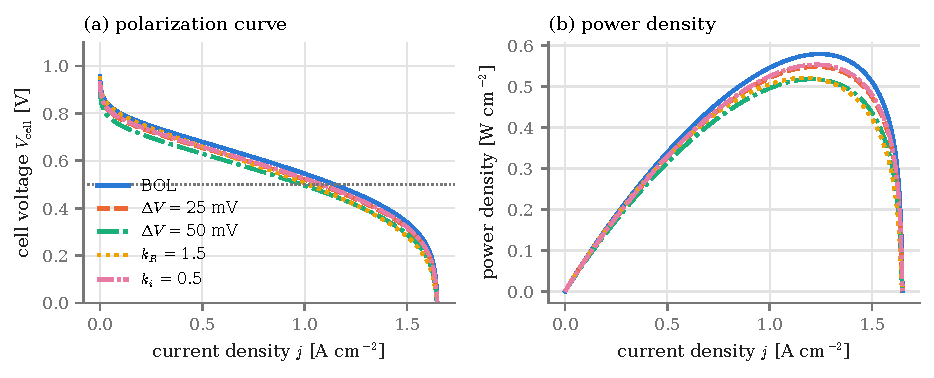
\includegraphics[width=\textwidth]{figures/fig_degradation_curves.pdf}
\caption{\code{PEMFC_GoodPerformance} at BOL and in four degraded states: polarization curve
(a) and power density (b). The dotted line in (a) marks the reference design voltage of
\SI{0.5}{V}.}
\label{fig:degcurves}
\end{figure}

\subsection{End-of-life sizing}

Setting \code{fc_voltage_loss}, \code{fc_ohmic_resistance_factor} or
\code{fc_exchange_current_factor} in the \code{EnergyConfig} of a design sizes the aircraft
at that state. \fn{SetInput} applies the state before the sizing loop. The stack then reaches
$\Vdes$ on the degraded curve, at a lower $\jdes$, and Eq.~\eqref{eq:area} gives a larger active
area. The mass per area of Eq.~\eqref{eq:mstack} stays referenced to the BOL curve, because the
stack specific power is a hardware figure. The end-of-life stack is therefore heavier. Sizing
the reference design at $\Delta V=\SI{50}{mV}$ (\fn{make_figures.py:group_eol}) gives the
results of Table~\ref{tab:eol}.

\begin{table}[ht]
\centering\small
\caption{Reference design sized at BOL and at end of life with $\Delta V=\SI{50}{mV}$.}
\label{tab:eol}
\begin{tabular}{@{}lrrr@{}}
\toprule
Quantity & BOL & EOL ($\Delta V$ = 50 mV) & change \\
\midrule
$\jdes$ [\si{A/cm^2}] & 1.147 & 0.987 & $-$14.0\,\% \\
active area [\si{m^2}] & 791 & 994 & +25.7\,\% \\
fuel-cell system [kg] & 2400 & 2882 & +20.1\,\% \\
hydrogen load [kg] & 450 & 517 & +15.0\,\% \\
peak heat [MW] & 4.70 & 5.55 & +18.1\,\% \\
TMS, Class I [kg] & 940 & 1110 & +18.1\,\% \\
$W_\mathrm{TO}$ [kg] & 21634 & 23400 & +8.2\,\% \\
\bottomrule
\end{tabular}
\end{table}

\subsection{Degraded flight of a sized aircraft}

A sized aircraft is flown degraded on a copy. The helper
\fn{examples/30_off_design_mission.py:fly_off_design(sized, range_nm, payload_kg=None, phi=None, state_of_health=None)}
deep-copies the design, applies \code{state_of_health} (a dictionary with the
\code{EnergyConfig} keys) through \fn{set_state_of_health}, resets the adequacy trackers and
closes the off-design take-off mass by a fixed-point iteration. It returns the trip fuel and a
list of violations and a list of risks. For the fuel cell it checks two things: that the
stack is never power-limited, and that the TMS can reject the heat (\fn{_tms_violation}). The
power limit is the maximum net power of the same polarization model that sized the stack, so
the fuel-cell power is not compared with the design mission peak: a stack sized on the
take-off or OEI floor can deliver more than that peak. With a Class-I TMS the peak heat over
the mission and the take-off point must not exceed the heat the TMS was sized for. With a
Class-II TMS the design hardware is checked at every point of the flown thermal profile and
of the flown mission (\fn{tms.CheckAtPoint}): a heat shortfall, a core pressure drop above its
budget or a choked duct is a violation, and a coolant-side wall below the coolant freezing
point is a risk.

Table~\ref{tab:degflight} flies the take-off-sized FC + battery design of example~30
(\fn{fc_battery_design}: $\varphi_\mathrm{TO}=0.15$, \SI{800}{m} field, \SI{1.5}{kW/kg} pack, battery
also on the taxi, sized at BOL, $W_\mathrm{TO}=\SI{24306}{kg}$) on its
nominal 750~nm mission in five states (\fn{make_figures.py:group_fcb}).

\begin{table}[ht]
\centering\small
\caption{Degraded flights of the example-30 design on its 750~nm mission. Trip hydrogen
includes the ground segments. Peak heat is compared with the TMS design heat of
\SI{5.338}{MW}. Load ratio: worst $\Pel/P_\mathrm{net,max}$ over the mission.}
\label{tab:degflight}
\setlength{\tabcolsep}{4pt}
\begin{tabular}{@{}lrrrrl@{}}
\toprule
State & trip H$_2$ [kg] & change & peak heat [MW] & load ratio & violations \\
\midrule
BOL & 374.6 & -- & 5.33 & 0.888 & none \\
$\Delta V$ = 25 mV & 394.1 & +5.2\,\% & 6.27 & 0.941 & TMS heat \\
$\Delta V$ = 50 mV & 418.3 & +11.7\,\% & 8.65 & 1.000 & TMS heat; fuel load; MTOW; \\
 & & & & & battery power \\
$k_R$ = 1.5 & 390.9 & +4.4\,\% & 7.33 & 0.991 & TMS heat \\
$k_i$ = 0.5 & 390.6 & +4.3\,\% & 6.08 & 0.931 & TMS heat \\
\bottomrule
\end{tabular}
\end{table}

The heat grows much faster than the hydrogen. A uniform loss of \SI{25}{mV} costs
\SI{5.2}{\percent} of hydrogen but raises the peak heat \SI{17}{\percent} above the TMS design
heat; \SI{50}{mV} raises it \SI{62}{\percent}. The reason is the ratio derived at the end of
Section~\ref{sec:heat}: at a given electrical power the hydrogen scales as $1/V_\mathrm{cell}$,
the heat as $(V_\mathrm{tn}-V_\mathrm{cell})/V_\mathrm{cell}$. The TMS, not the tank, is
therefore the first constraint to bind. At \SI{50}{mV}, which is \SI{10}{\percent} of the
\SI{0.5}{V} design voltage, the stack reaches its power limit (worst load ratio 0.99996, just
below the flag threshold), and the heavier off-design aircraft also exceeds the MTOW, the
design fuel load and the battery power capability. The ohmic drift $k_R=1.5$ costs less
hydrogen than \SI{25}{mV}, but more heat, because it acts most at the high-current climb and
take-off points that set the peak heat.

\subsection{Duty cycle of a take-off-sized stack}

Degradation depends on how the stack is loaded. Vichard et al.~\cite{vichard} note that the
load variations and start-stop conditions of a vehicle significantly affect durability. Pessot
et al.~\cite{pessot} estimate the cell-voltage degradation of a mission profile by superposing
the degradations measured for its quasi-static and dynamic sub-missions. Both approaches need
the duty of the stack, and in PhlyGreen the duty is set by the sizing. Figure~\ref{fig:duty} gives the time spent in each band of $j/\jdes$ by the same
example-30 design on its nominal mission (diversion not flown), on a \SI{2}{s} grid, plus the
ground segments.

\begin{figure}[ht]
\centering
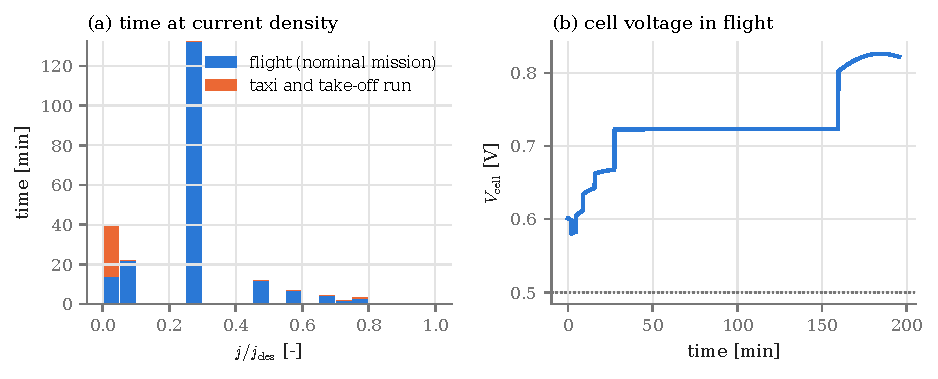
\includegraphics[width=\textwidth]{figures/fig_duty_histogram.pdf}
\caption{Duty of the example-30 design (take-off-sized FC + battery, BOL): time at current
density, as a fraction of the design current density (a), and in-flight cell voltage (b). The
flown nominal mission lasts \SI{195.6}{min}; taxi \SI{26}{min}; take-off run \SI{0.7}{min}.}
\label{fig:duty}
\end{figure}

The stack spends \SI{79}{\percent} of the \SI{195.6}{min} flight between \SI{5}{\percent} and
\SI{30}{\percent} of $\jdes$, at cell voltages from 0.72 to \SI{0.82}{V}, and \SI{36}{min}
above \SI{0.80}{V}. It never exceeds \SI{77}{\percent} of $\jdes$ in flight. The take-off run
reaches \SI{75}{\percent} of $\jdes$ (\SI{0.585}{V}). The 26 minutes of taxi run at
\SI{4.4}{\percent} of $\jdes$ and \SI{0.829}{V}. Over the whole profile, diversion included (\SI{257.7}{min}), the
same quantities are \SI{78}{\percent} and \SI{49.5}{min}; these are the values quoted in the user
guide. A take-off-sized stack therefore runs at low load and high cell voltage for most of its
life. The model does not quantify what this regime
does to the degradation rate.

\subsection{Hook for ageing estimators}

An ageing estimator needs the operating point along the mission. \fn{ComputePRatio} exposes it
after every call: $j$ (\code{i_op_last}), $V_\mathrm{cell}$ (\code{v_cell_last}),
$\eta_\mathrm{FCS}$ (\code{eta_fcs_last}), heat and flows. The integrator solutions in
\code{mission.integral_solution} give time and $\beta$. Re-evaluating \fn{ComputePRatio} on a
time grid, as \fn{make_figures.py:mission_history} does on a copy of the aircraft, yields the
duty of Figure~\ref{fig:duty}. The ground segments are not in \code{integral_solution}; their
operating point follows from one call at the take-off condition with the taxi and take-off
powers of \fn{Mission._ground_segments}. An estimator would map this duty to a $\Delta V$ (or
to $k_R$, $k_i$) and feed it back through \fn{set_state_of_health} or the \code{EnergyConfig}
fields. No such estimator is part of the package.

%% =====================================================================================
\section{Usage}
\label{sec:usage}

This section shows how to set up, run and read a fuel-cell design. All snippets run from
\fn{trunk/} in the \code{phlygreen} environment; we ran each of them and quote their output.

\subsection{Inputs}
\label{sec:inputs}

Table~\ref{tab:inputs} lists every fuel-cell input. The typed field belongs to
\code{EnergyConfig} unless marked otherwise; the legacy key is the \code{EnergyInput} (or
\code{MissionInput}) dictionary key that \code{ReadInput} receives. ``req.'' marks inputs that
\fn{FuelCell.SetInput} requires: a missing one raises \code{FuelCellError}.
\fn{examples/common.py:_energy_hydrogen} and \fn{_mission} write every one of these inputs
explicitly at the values used in this manual, so they are a convenient template. The helper
\fn{common.tms_config(tms_class)} does the same for the TMS, and \fn{hydrogen_config} and
\fn{fuelcell_battery_config} accept \code{tms_class='I'} or \code{'II'} to attach it
(\code{None} keeps the Class-I default).

\begingroup\small
\setlength{\tabcolsep}{4pt}
\begin{longtable}{@{}p{3.6cm}p{3.6cm}p{1.9cm}p{1.1cm}p{4.3cm}@{}}
\caption{Fuel-cell inputs: typed field, legacy dictionary key, default, units and meaning.}
\label{tab:inputs}\\
\toprule
Config field & Legacy key & Default & Units & Meaning \\
\midrule
\endfirsthead
\toprule
Config field & Legacy key & Default & Units & Meaning \\
\midrule
\endhead
\bottomrule
\endfoot
\code{Ef} & \code{Ef} & req. & J/kg & hydrogen specific energy; must be the HHV, \num{141.87e6} \\
\code{fc_model} & \code{Model} & req. & -- & key of \code{FC_Database} \\
\code{v_cell_design} & \code{V Cell Design} & req. & V & design cell voltage $\Vdes$ \\
\code{i_rated} & \code{i Rated} & req. & \si{A/cm^2} & fallback, only if $\Vdes$ is not on the curve \\
\code{stack_power_density} & \code{Stack Power Density} & req. & W/kg & stack specific power at \SI{0.7}{V}, BOL \\
\code{bop_mass_ratio} & \code{BoP Mass Ratio} & req. & -- & BoP mass / stack mass \\
\code{eta_pmad} & \code{Eta PMAD} & req. & -- & PMAD efficiency \\
\code{eta_electric_motor} & \code{Eta Electric Motor} & req. & -- & motor efficiency \\
\code{eta_gearbox} & \code{Eta Gearbox} & req. & -- & gearbox efficiency \\
\code{eta_propulsive} & \code{Eta Propulsive} & 0.8 & -- & propeller efficiency \\
\code{eta_electric_motor_model} & \code{Eta Electric Motor Model} & constant & -- & \code{'Smart'}: d-q motor model \\
\code{stack_design_voltage} & \code{Stack Design Voltage} & 1000 & V & bus voltage; sets $N_\mathrm{cells}$ only \\
\code{specific_power_powertrain} & \code{Specific Power Powertrain} & [--, 5000] & W/kg & 2nd entry: motor \\
\code{specific_power_pmad} & \code{Specific Power PMAD} & 10000 & W/kg & PMAD \\
\code{fc_product_water_vapour_fraction} & \code{FC Product Water Vapour Fraction} & \code{'auto'} & -- & $x_v$, or computed \\
\code{fc_cathode_inlet_rh} & \code{FC Cathode Inlet RH} & 0.0 & -- & humidifier $\phi_\mathrm{hum}$ at $T_\mathrm{op}$ \\
\code{fc_ambient_relative_humidity} & \code{FC Ambient Relative Humidity} & 0.0 & -- & weather: ambient $\phi_a$ \\
\code{fc_voltage_loss} & \code{FC Voltage Loss} & 0.0 & V & $\Delta V$ \\
\code{fc_ohmic_resistance_factor} & \code{FC Ohmic Resistance Factor} & 1.0 & -- & $k_R$ \\
\code{fc_exchange_current_factor} & \code{FC Exchange Current Factor} & 1.0 & -- & $k_i$ \\
\code{h2_fuel_margin} & \code{H2 Fuel Margin} & 0.05 & -- & extra hydrogen loaded \\
\code{h2_gravimetric_index} & \code{H2 Gravimetric Index} & 0.35 & -- & tank index if no LH2 tank \\
\code{contingency_fuel} & \code{Contingency Fuel} & 5\,\% load & kg & final reserve \\
\code{hex_specific_power_h2} & \code{HEX Specific Power H2} & 5000 & W/kg & Class-I TMS \\
\code{battery_specific_energy} & \code{Battery Specific Energy} & 250 & Wh/kg & FC + battery, Class I \\
\code{battery_specific_power} & \code{Battery Specific Power} & 1500 & W/kg & FC + battery, Class I \\
\code{battery_usable_soc} & \code{Battery Usable SOC} & 0.8 & -- & FC + battery, Class I \\
\midrule
\multicolumn{5}{@{}l}{\code{MissionConfig}} \\
\code{taxi_out_time}, \code{taxi_in_time} & \code{Taxi Out Time}, \code{Taxi In Time} & 13, 13 & min & ground segments \\
\code{taxi_power_fraction} & \code{Taxi Power Fraction} & 0.07 & -- & of take-off-field power \\
\code{takeoff_time} & \code{Takeoff Time} & 0.7 & min & take-off run \\
\code{takeoff_power_fraction} & \code{Takeoff Power Fraction} & 1.0 & -- & of take-off-field power \\
\code{taxi_phi} & \code{Taxi Supplied Power Ratio} & take-off $\varphi$ & -- & battery share in taxi \\
\code{disa} & \code{DISA} & 0 & K & mission ISA deviation \\
\midrule
\multicolumn{5}{@{}l}{\code{TankConfig} (\code{TankInput}) and \code{TMSConfig} (\code{TMSInput})} \\
\code{max_diameter} & \code{Max Diameter} & req. & m & LH2 tank outer diameter \\
\code{number_of_tanks} & \code{Number of Tanks} & 1 & -- & \\
\code{tank_model} & \code{Tank Model} & \code{Svensson_Default} & -- & key of \code{TANK_Database} \\
\code{tms_class} & \code{TMS Class} & \code{'I'} & -- & see the TMS manual; \fn{common.tms_config} writes every field \\
\end{longtable}
\endgroup

Table~\ref{tab:constants} lists the model constants that are hard-coded as attributes or
literals. They are model assumptions; none has a source in the repository other than the code
comments quoted in this manual.

\begin{table}[ht]
\centering\small
\caption{Hard-coded constants of \fn{FuelCell.py}.}
\label{tab:constants}
\setlength{\tabcolsep}{4pt}
\begin{tabular}{@{}llr@{}}
\toprule
Constant & Code & Value \\
\midrule
fixed auxiliary load, fraction of $P_\mathrm{fc,rated}$ & \code{Fixed_Aux_Load} & 0.015 \\
compressor / turbine isentropic efficiency & \code{comp_eta}, \code{turb_eta} & 0.75 / 0.70 \\
air stoichiometric ratio $\lambda$ & \code{stoich} & 2.0 \\
air mass flow per ampere per cell at $\lambda=1$ & literal & \SI{3.57e-7}{kg/(A.s)} \\
turbine inlet pressure / cathode pressure & literal & 0.95 \\
gross-power sizing allowance $\eta_\mathrm{BoP,s}$ & \code{BoP_Power_Sizing_Efficiency} & 0.85 \\
power sizing margin & \code{SizingMargin} & 1.0 \\
stack mass reference voltage & literal & \SI{0.7}{V} \\
minimum number of cells & literal & 100 \\
bounds of $\eta_\mathrm{total}$ & literal & [0.01, 0.85] \\
operating-point grid & literal & 50 points, \SI{e-4}{}--$0.95\,j_\mathrm{lim}$ \\
seed power-to-weight floor, seed mass & literal & \SI{155}{W/kg}, \SI{25000}{kg} \\
\bottomrule
\end{tabular}
\end{table}

\subsection{Sizing a hydrogen aircraft with the typed API}

\begin{lstlisting}
import sys
sys.path.insert(0, "examples")          # run from trunk/
import PhlyGreen as pg
from common import hydrogen_config

cfg = hydrogen_config(v_cell_design=0.5)   # typed AircraftConfig
cfg.energy.stack_design_voltage = 800.0    # optional: bus voltage [V]
aircraft = pg.build_aircraft()
aircraft.configure(cfg)                    # ReadInput + FindDesignPoint + WeightEstimation

r = aircraft.results()                     # AircraftResults dataclass
fc = aircraft.fuelcell
print(f"WTO {r.WTO:.0f} kg, FC system {r.WPT:.0f} kg, rating {r.fuelcell_rating/1e6:.2f} MW")
print(f"N_cells {fc.N_cells}, A_cell {fc.A_cell_reale:.0f} cm2, j_des {fc.i_max_density:.3f} A/cm2")
print(fc.report_sizing()["status"])
\end{lstlisting}
The output is \code{WTO 21634 kg, FC system 2400 kg, rating 3.85 MW}, then
\code{N_cells 1600, A_cell 4942 cm2, j_des 1.147 A/cm2} and \code{ok}. Compared with
Table~\ref{tab:refdesign}, the lower bus voltage changed the cell count and the cell area and
nothing else. The legacy dictionary API is equivalent: \code{cfg.energy.to_dict()} returns the
\code{EnergyInput} dictionary with the keys of Table~\ref{tab:inputs}.

\paragraph{Reading the results.} \code{aircraft.results()} returns, among others,
\code{WTO}, \code{WPT}, \code{Wf}, \code{fuelcell_rating}, \code{tank_mass}
(\code{weight.WTank}), \code{hex_mass} and \code{tms_mass} (both \code{weight.WHeat_Exchanger}
for the fuel-cell configurations: the fuel-cell TMS, plus the heat exchanger of a Class-II
battery), \code{TO_PP} and \code{Max_PEng}. Its \code{empty_weight} is every closure mass that
is not payload or fuel: structure, fuel-cell system, crew, battery, hydrogen tank and heat
exchangers, so that \code{empty_weight} + \code{WPayload} + \code{Wf} + reserve $=W_\mathrm{TO}$.
The useful attributes are on the subsystems:
\code{aircraft.weight.WH2_Fuel}, \code{WTank}, \code{WHeat_Exchanger}, \code{WBat};
\code{aircraft.fuelcell.N_cells}, \code{A_cell_reale}, \code{P_fc_rated},
\code{i_max_density} ($\jdes$), \code{x_vapour}; and \code{aircraft.mission.TO_PP},
\code{Max_PEng}, \code{TO_FC_Thermal_Pwr}, \code{TO_P_H2_Thermal}, \code{Max_FC_Thermal_Pwr},
\code{thermal_profile}, \code{integral_solution}.

\subsection{Evaluating one operating point}

\begin{lstlisting}
import copy
fc = copy.deepcopy(aircraft.fuelcell)      # ComputePRatio has side effects
fc.reset_adequacy()
pratio = fc.ComputePRatio(8000.0, 125.0, 1.5e6)   # altitude [m], TAS [m/s], P_prop [W]
print(f"H2 power / propulsive power = {pratio[0]:.3f}")
print(f"j = {fc.i_op_last:.3f} A/cm2, V = {fc.v_cell_last:.3f} V, "
      f"eta_FCS = {fc.eta_fcs_last:.3f}, Q = {fc.Q_thermal/1e6:.2f} MW, "
      f"mdot_H2 = {fc.mdot_h2*1e3:.1f} g/s, limited = {fc._power_limited}")
\end{lstlisting}
On the reference design this prints a ratio of 2.982, then $j=\SI{0.382}{A/cm^2}$,
$V=\SI{0.710}{V}$, $\eta_\mathrm{FCS}=0.432$, $\dot Q=\SI{1.64}{MW}$,
$\dot m_{\mathrm{H_2}}=\SI{31.5}{g/s}$ and \code{limited = False}. Work on a copy: the call
overwrites the stored operating point and the adequacy trackers of the design.

\subsection{Sweeps and outer loops}

\begin{lstlisting}
def set_voltage(cfg, v):
    cfg.energy.v_cell_design = float(v)

base = hydrogen_config()
for v in (0.50, 0.60):
    res = pg.evaluate(base, set_voltage, v)     # fresh aircraft, base not mutated
    print(v, round(res.WTO), round(res.WPT))
print(round(pg.run_design(base).WTO))
\end{lstlisting}
This prints \code{0.5 21634 2400}, \code{0.6 22032 2748} and \code{21634}.
\fn{pg.run_design} and \fn{pg.evaluate} (\fn{PhlyGreen/api.py}) build a fresh aircraft for
every call and never mutate the input, so they are safe in loops and in parallel. A design
takes about \SI{15}{s} with the Class-I TMS and up to about a minute with the Class-II TMS.

\subsection{End-of-life sizing and degraded flight}

\begin{lstlisting}
cfg = hydrogen_config()
cfg.energy.fc_voltage_loss = 0.05            # size the aircraft at end of life
eol = pg.run_design(cfg)

import importlib.util
spec = importlib.util.spec_from_file_location("ex30", "examples/30_off_design_mission.py")
ex30 = importlib.util.module_from_spec(spec); spec.loader.exec_module(ex30)
sized = ex30.fc_battery_design()             # FC + take-off battery, 800 m field
rng = sized.MissionInput["Range Mission"]    # 750 nm
for soh in ({}, {"fc_voltage_loss": 0.025}, {"fc_ohmic_resistance_factor": 1.5}):
    r = ex30.fly_off_design(sized, rng, state_of_health=soh)
    print(soh, f"trip H2 {r.trip_fuel:.1f} kg", r.violations)
\end{lstlisting}
The loop reproduces the first, second and fourth rows of Table~\ref{tab:degflight}. The design
object \code{sized} is not modified.

\subsection{Pitfalls}

\begin{itemize}
  \item \textbf{Wrong heating value.} \code{Ef} must be \SI{141.87e6}{J/kg} (HHV); see
  Section~\ref{sec:netpower}.
  \item \textbf{Power-limited at altitude.} The available net power falls with altitude
  (Figure~\ref{fig:efficiency}). A stack sized with a smaller allowance, or flown on a profile
  with a high-altitude power peak, can be power-limited even if its sea-level rating looks
  sufficient. \fn{DesignAircraft} warns through \fn{report_sizing}; check
  \code{fc.report_sizing()['status']} in scripts and sweeps.
  \item \textbf{Short missions are rejected by the profile.} A \code{ConstantMachCruise} fills
  the range left by the climbs and descents of its phase. If they exceed the phase range,
  \fn{Profile} raises a \code{ValueError} (``the cruise would have a negative length''). With
  the climb to \SI{8000}{m} of \fn{common.py}, example~30 notes that ranges below about 210~nm
  have no cruise.
  \item \textbf{Design does not close.} A high design voltage or a low stack specific power
  makes the power-proportional masses snowball, and \fn{Weight.Hydrogen} raises a
  \code{RuntimeError}. Over-demanding constraints are amplified in the same way.
  \item \textbf{\code{i_rated} is a fallback only.} It has no effect for design voltages on
  the curve (Section~\ref{sec:design}). To enlarge an undersized stack, the
  \fn{report_sizing} warning suggests raising \code{FuelCell.SizingMargin} or the design
  cell voltage.
  \item \textbf{Two temperature deviations.} \code{MissionConfig.disa} sets the flown mission:
  the flight performance, the fuel-cell ambient state and the TMS ram air.
  \code{ConstraintsConfig.disa} sets the constraint diagram and the take-off and OEI speeds
  of the off-mission sizing points. A hot-day design sets both. \fn{Mission.SetInput} writes
  \code{mission.DISA} from the input, so a value assigned by hand before \code{configure} is
  overwritten; assign it after the design to fly an off-design mission.
  \item \textbf{Side effects.} \fn{ComputePRatio} and \fn{EvaluateMission} overwrite stored
  state. Use \code{copy.deepcopy} before probing a sized aircraft, and call
  \fn{reset_adequacy} before a new mission.
\end{itemize}

%% =====================================================================================
\section{Verification}
\label{sec:verification}

This section lists the tests that pin the fuel-cell behaviour and the limitations of the model.
The tests live in \fn{trunk/tests/}; those marked \code{slow} run full designs and are skipped
by \code{pytest -m "not slow"}.

\begin{table}[ht]
\centering\small
\caption{Tests that pin the fuel-cell behaviour.}
\label{tab:tests}
\begin{tabularx}{\textwidth}{@{}p{5.4cm}X@{}}
\toprule
Test (file: function) & What it pins \\
\midrule
\fn{regression/test_hydrogen.py} & polarization curve decreasing in $j$; sizing sets geometry and a positive mass; $\eta_\mathrm{FCS}$ a sensible fraction; design closes and the mass breakdown sums to $W_\mathrm{TO}$ (slow); stack covers mission peak and take-off/OEI (slow); design voltage changes the design (slow) \\
\fn{regression/test_fuelcell_sizing.py} & auto-sized stack is not power-limited; a stack shrunk to \SI{45}{\percent} of \code{TO_PP} is reported \code{'UNDERSIZED'} with a warning and \code{min_rating} above the rating (slow) \\
\fn{unit/test_fuelcell_heat.py} & Antoine saturation pressure; $x_v=1$ for dry air at \SI{80}{\celsius}, \SI{1.5}{bar}; $x_v=0$ for saturated inlet; $x_v$ falls with humidity and pressure; $x_v=1$ above the boiling point; thermoneutral voltages \\
\fn{regression/test_fuelcell_battery.py} & configuration valid; both sources used; no battery at $\varphi=0$; battery grows with $\varphi$; default battery is Class I; Class-II pack sized; battery power flows through the motor and PMAD masses (slow) \\
\fn{regression/test_fc_battery_takeoff_assist.py} & take-off battery does not pay on \SI{1107}{m}; on \SI{800}{m} $0.1<\varphi^*<0.2$, the stack shrinks, the motor does not, and the default pack does not pay; an assumed \SI{3}{kW/kg} pack on the take-off run only makes the aircraft lighter (slow) \\
\fn{regression/test_degradation.py} & $\Delta V$ shifts the curve and the BOL curve stays available; parameter drift lowers the curve and resets; inputs validated and read; power-limited branch continuous and monotone in demand and degradation (slow); EOL sizing enlarges stack and TMS (slow); degraded flight reports the TMS heat violation and leaves the design unchanged (slow) \\
\fn{regression/test_fuelcell_air_system.py} & exhaust mass balance; the expander works on the exhaust, not on air; ambient humidity reaches the cathode; the mission DISA input reaches \code{mission.DISA} and the fuel-cell ambient; a hot day changes the hydrogen design \\
\fn{regression/test_degradation.py} (mission accounting) & the running stack burns hydrogen at zero propulsive power; the FC + battery chain includes the propeller; battery energy and power are terminal quantities; degraded flight rates the Class-II TMS hardware \\
\fn{regression/test_hydrogen_tank.py} & LH2 tank sizing, self-pressurisation, venting, heater, tracked mission (CoolProp) \\
\bottomrule
\end{tabularx}
\end{table}

\subsection{Modelling assumptions and limitations}
\label{sec:limitations}

\paragraph{Model assumptions.}
\begin{itemize}
  \item Quasi-steady operation: no stack thermal or electrochemical dynamics, no start-up.
  \item Constant cathode pressure at every altitude; no pressure or stoichiometry scheduling.
  \item The polarization curve does not depend on temperature or humidity.
  \item Constant compressor and turbine efficiencies and molar heat capacities; the expander
  inlet is at $T_\mathrm{op}$; the liquid product water is separated before the expander; no
  motor or inverter loss in the air system; dry-air $c_p$ for the humid compressor flow.
  \item Constant fixed auxiliary load, \SI{1.5}{\percent} of the rating, at every load.
  \item Stack mass per area from a specific power at \SI{0.7}{V}, BOL; BoP mass proportional to
  stack mass.
  \item $x_v$ is an equilibrium upper bound at the stack exit; no system-level water balance.
  \item The battery assists the OEI climb with the take-off share.
  \item In \code{'FuelCellBattery'} a Class-II motor or propeller model is read at the power of
  each branch, not at the total power through the shared drive.
  \item No ageing estimator: the state of health is an input.
\end{itemize}


\section*{Reproducing this manual}

From \fn{trunk/}, \code{python ../manuals/fuel-cell/scripts/make_figures.py} in the \code{phlygreen} environment
regenerates every figure and writes every quoted number to
\fn{manuals/fuel-cell/figures/manual_numbers.json} (about 40 minutes in total, of which the take-off-assist group of example~23 takes about 30; each group can be run alone by naming it on the command line). Then, from
\fn{manuals/fuel-cell/}, \code{latexmk -pdf -interaction=nonstopmode -outdir=build fuelcell_manual.tex}.



\begin{thebibliography}{9}
\bibitem{kulikovsky} A.~A.~Kulikovsky, \emph{A physically-based analytical polarization curve
of a PEM fuel cell}, Journal of the Electrochemical Society 161(3) (2014) F263--F270. 
\bibitem{massaro} M.~C.~Massaro et al., \emph{Optimal design of a hydrogen-powered fuel cell
system for aircraft applications}, Energy Conversion and Management 306 (2024) 118266.
\bibitem{park2025ohv} S.~Park et al., \emph{Effects of water evaporation and condensation on 
the operating heating value and system efficiency of polymer electrolyte membrane
fuel cells: Temperature-dependent phase separation modeling}, Chemical Engineering Journal 516 (2025) 163864.
\bibitem{svensson} C.~Svensson et al., \emph{Modelling hydrogen fuel cell aircraft in SUAVE},
ICAS 2024. Source of \fn{TANK_Database.py}.
\bibitem{pessot} A.~Pessot et al., \emph{Development of an aging estimation tool for a PEM
fuel cell submitted to a mission profile}, Fuel Cells 20 (2020) 253--262. 
\bibitem{vichard} L.~Vichard, N.~Yousfi Steiner, N.~Zerhouni, D.~Hissel, \emph{Hybrid fuel cell
system degradation modeling methods: a comprehensive review}, Journal of Power Sources 506
(2021) 230071.
\end{thebibliography}

\end{document}
